\documentclass{cshonours}
\usepackage{thesis, hyperref, graphics, float}

\title{Refinement Operators for Doxastic and Epistemic Logics}
\author{James Hales}
\keywords{Epistemic Logic, Refinement Quantification, Axiomatizations, Decision Procedures.}
\categories{}

\begin{document}

\maketitle

% Abstract
% Acknowledgements
% Introduction
% Literature review
% K
% - Translation
% - Tableau
% - Brute force (?)
% S5/KD45
% - Translation
% - Tableau
% - Brute force (? / single-agent)
% - Axiomatisation

\begin{acknowledgements}
First and foremost I would like to thank my supervisors, Tim French and Rowan
Davies. Tim and Rowan have had a remarkable level of involvement in my honours
project, supporting me greatly in the last year with frequent meetings and
proof-readings of draft papers. It's thanks to them that, in my honours year I
submitted a paper to the Methods for Modalities conference in Osuna, Spain,
which was ultimately accepted for publication, an experience that has further
motivated me to pursue a career in academia. Tim and Rowan must have reviewed
dozens of draft copies of my paper and thesis, providing helpful feedback each
time, and I am truly grateful for the investment of time that they have both
made in supervising my honours project. I would also like to acknowledge the
financial support that Tim and Rowan have granted me, which has allowed me to
attend the conference in Osuna.

I would like to thank John Slaney and Rajeev Gor\'{e} of the Australian National
University, for the Logic Summer School that I attended in 2010. John Slaney
organises the Logic Summer School at ANU each year, and it was thanks to him and
the Australian National University that I received funding to attend the summer
school, where I received my first in-depth introduction to logic. Rajeev
Gor\'{e} in particular gave me my first course in modal logic, from which I
gained a lot, and Rajeev also offered me advice about the topic of my honours
thesis, which I ultimately followed.

I would also like to thank Hans van Ditmarsch, and the anonymous reviewers of
the Methods for Modalities conference that I submitted a paper to this year.
Much of the recommendations that I received from the reviewers, and also from
Hans, has made it into this thesis.

Finally I would like to acknowledge the financial support of the Hackett
Foundation for the Hacket Foundation Alumni Honours Scholarship, which has made
my life easier in the last year, and has partly funded my trip to Osuna for the
Methods for Modalities conference.
\end{acknowledgements}

\begin{abstract}
Modal logics are extensions of propositional logic, with which one can qualify
the truth of statements with operators known as modalities. Epistemic logic is a
variant of modal logic, commonly known as the logic of knowledge. Modalities in
epistemic logic qualify statements by saying that a particular agent knows a
statement to be true. Thus epistemic logic can be used to reason about the
knowledge of a collection of agents. Doxastic logic is a similar logic, used to
reason about beliefs rather than knowledge.

Informative updates are events that provide agents in modal settings with
additional information. The effect of an informative update may be to give new
knowledge or beliefs to the agents in the system. Informative updates in an
epistemic setting can be modelled by the refinements of a Kripke model in modal
logic.

Refinement quantifiers are introduced to variants of modal logic to produce
refinement quantified modal logics. The refinement quantifiers are operators
that quantify over the refinements of a Kripke model, and as these refinements
model informative updates, this quantification can be said to be equivalent to
quantifying over the informative updates that are possible in a Kripke model.
Recent work by van Ditmarsch, French and Pinchinat~\cite{french2010future} has
presented an axiomatisation and decidability results for the single-agent
refinement quantified modal logic. We extend these results to apply to the
single-agent doxastic and epistemic logics, and to the multi-agent modal and
doxastic logics.
\end{abstract}

\tableofcontents
\chapter{Introduction}

% Introduce modal logic

{\em Modal logics} are extensions of propositional logic, used to reason about
the properties of relational structures known as {\em Kripke models}, by
qualifying the truth of statements with operators known as {\em modalities}.
{\em Epistemic logic} is a variant of modal logic, commonly known as the logic
of knowledge, where the Kripke models that are considered encode the knowledge
that a collection of agents hold about the state of the world, and the effect of
modalities is to say that an agent {\em knows} a statement to be true. {\em
Doxastic logic} is a similar variant of modal logic, the logic of belief, that
considers the beliefs that a collection of agents hold. The difference between
the notions of knowledge and belief used in epistemic and doxastic logics is
simply that anything that an agent knows must be true, whereas it is permissible
for an agent to believe something that is false.

% Introduce dynamic epistemic logic
{\em Dynamic epistemic logic} and {\em dynamic doxastic logic} are fields that
consider how the knowledge or beliefs of a collection of agents may change in
response to {\em informative updates}. Informative updates are events, such as
messages or announcements, that communicate new information to agents. 
Informative updates change the knowledge or beliefs of agents, whilst leaving
the {\em factual} information about the state of the world unchanged.  These
fields consider questions such as what knowledge or belief states can result
from specific informative updates, and how or whether a specific knowledge or
belief state can be achieved from a series of arbitrary informative updates,
perhaps with restrictions on what kinds of informative updates are allowed.

% Muddy children example
A classic example is that of the muddy children puzzle, explained by van
Ditmarsch, van der Hoek and Kooi~\cite{vanditmarsch2007dynamic}:

\begin{quote}
``A group of children has been playing outside and are called back into the house
by their father. The children gather round him. As one may imagine, some of them
have become dirty from the play and in particular: they may have mud on their
forehead. Children can only see whether other children are muddy, and not if
there is any mud on their own forehead. All this is commonly known, and the
children are, obviously, perfect logicians. Father now says: “At least one of
you has mud on his or her forehead.” And then: “Will those who know whether they
are muddy please step forward.” If nobody steps forward, father keeps repeating
the request.''
\end{quote}

The puzzle is whether each of the children can eventually determine whether
they are muddy or not. The children are not allowed to communicate with one
another, except by stepping forward when they know whether they are muddy or
not. It can be shown that if there are $m$ muddy children, those children will
step forward after the father has asked his question $m$ times, at which point
the remaining children will know that they are not muddy, and so they too will
step forward the next time the father asks his question.

The muddy children puzzle demonstrates how agents in an epistemic system can
gain knowledge about the state of the world indirectly. In the case of $m$ muddy
children, the first $m - 1$ times that the father asks his question, no child
steps forward, and so the only information that is given is that none of the
children knows whether or not they are muddy. Despite begin given the same
information over and over, that does not directly provide any information about
whether the children are muddy or not, this is enough for each child to
eventually determine whether or not they are muddy, and this fact is surprising.

% Motivate dynamic epistemic logic
Problems of this form motivates our research into dynamic epistemic logic and
dynamic doxastic logic; we wish to know whether it is possible for agents to
achieve certain knowledge or belief states after some sequence of informative
updates. This is an interesting question because, as we have already
demonstrated with the muddy children puzzle, it is not always obvious whether or
not certain knowledge or belief states are attainable. This has applications in
areas such as games with imperfect information, where one may wish to know
whether certain knowledge can be deduced from given information, or in security
protocols, where one may desire assurances that certain knowledge cannot be
indirectly deduced from seemingly innocuous communication.

% Introduce informative updates
Previous work has considered a number of different representations of
informative updates. In the context of epistemic logic, two of the most notable
are {\em public announcements}, and {\em action models}. Public announcements
are a relatively simple and restrictive form of informative update, whereas
actions models are more general and expressive. We avoid discussing
representations in doxastic logic for the time being, as the most notable,
belief revision, is conceptually different from the epistemic notions of
information change that the present work is based on.

% Motivate previous logics
As we are interested in questions about what knowledge or belief states can
result from informative updates, we consider extensions of epistemic or doxastic
logics that allow us to reason about this. There are two main directions that we
can take with such extensions. The first is logics with which we can reason
about the results of {\em specific} informative updates; in such a logic we can
say of some specific informative update that ``after the informative update
$\phi$, the statement $\psi$ is true in the resulting knowledge state''. The
second is logics with which we can reason about the results of {\em arbitrary}
informative updates, by quantifying over them; in such a logic we can say
that ``there exists an informative update after which $\psi$ is true in the
resulting knowledge state''.

% Introduce PAL, AML, and APAL
The {\em public announcement logic}, introduced by
Plaza~\cite{plaza2007logics}, and also independently by Gerbrandy and
Groenvald~\cite{gerbrandy1997reasoning} is an extension of epistemic logic that
introduces an operator for reasoning about the results of a specific public
announcement. A similar logic, the {\em action model logic}, was introduced by
Baltag and Moss~\cite{baltag2004logics}, allows reasoning about the results of
executing a specific action model. Balbiani, et
al.~\cite{balbiani2007arbitrary} then explored the {\em arbitrary public
announcement logic}, an extension of the public announcement logic that adds an
operator for reasoning about the results of arbitrary public announcements.  It
was later shown by van Ditmarsch and French~\cite{french2008undecidability}
that the arbitrary public announcement logic is undecidable. It has not been
considered whether a similar extension of action model logic would be decidable
or not, but the effect of the undecidability result in arbitrary public
announcement logic has been to encourage research into weaker versions of this
logic that are more likely to be decidable.

% Introduce FEL
The {\em future event logic}, introduced by van Ditmarsch and
French~\cite{french2009simulation} is an extension of epistemic logic that
introduces an operator for quantifying over the {\em refinements} of a Kripke
model. The finite refinements of a Kripke model can be shown to correspond to
the results of executing arbitrary action models on that Kripke model, and so
the effect of quantifying over the refinements of a Kripke model can reasonably
be said to be equivalent to quantifying over arbitrary informative updates. van
Ditmarsch, French and Pinchinat~\cite{french2010future} previously gave an
axiomatisation and decidability results for a simplified version of this logic,
in the context of single-agent modal logic, as opposed to multi-agent epistemic
logic.

% The present work
The present work extends the future event logic to the setting for which it was
originally intended: epistemic logic. For this paper we will refer to the future
event logic using the more up to date and general name of {\em refinement
quantified modal logics}. We consider refinement quantified versions of modal,
doxastic and epistemic logics. We provide axiomatisations for the refinement
quantified epistemic and doxastic logics in the single-agent case, and provide
axiomatisations for the refinement quantified modal and doxastic logics in the
multi-agent case. As our axiomatisations involve translating the refinement
quantified logics into basic modal logics, this gives us decidability results,
and upper bounds on the complexities of these logics, amongst other results.

\chapter{Technical preliminaries}

% Introduction to modal logic
As has been said earlier, modal logic is used to reason about the intrinsic
properties of Kripke models. Under the {\em possible worlds} interpretation of
modal logic, a Kripke model is said to encode information about the possible
ways that the world could be, with respect to a specific set of facts modelled
as propositional atoms. If we use the analogy of knowledge, then we can view the
possible worlds as a way to represent the notion of imperfect knowledge. If an
agent knew everything that there was to know about the world, then they would
only consider one world possible: the actual world; whereas, if an agent was
unsure about some fact $p$, then the agent would consider at least two worlds
possible: the world where $p$ is true, and the world where $p$ is false.

Modal logics allow us to reason about these possible worlds by qualifying
statements with operators known as modalities. If we are considering a
multi-agent setting, where there is a set $A$ of agents, then modal logic
introduces the operators $\knows_a$ and $\suspects_a$ for each agent $a \in A$.
We can qualify a statement $\phi$ with these operators, where $\knows_a \phi$
means that $\phi$ is true in every world that the agent $a$ considers possible,
and $\suspects_a \phi$ is true in at least one of the worlds that the agent $a$
considers possible. In basic modal logic, the operator $\knows_a$ is said to
represent necessity; $\knows_a \phi$ means that $a$ considers $\phi$ to be
necessarily true. In doxastic and epistemic logic on the other hand, $\knows_a$
is said to represent belief and knowledge respectively.

In this chapter we will provide some of the technical preliminaries that are
required throughout this paper. We give a short introduction to modal, doxastic
and epistemic logics, and give the definition of a refinement that is used by
the future event logic. We also give some useful results that we refer to later
in the paper.

We begin with the definition of a Kripke model, the definition of the modal
language \lang{}, and the semantics of modal logic.

% Definition of Kripke models
Let $A$ be a non-empty, finite set of agents, and let $P$ be a non-empty,
countable set of propositional atoms.

\begin{definition}[Kripke model]
A \textit{Kripke model} $M = (S, R, V)$ consists of a \textit{domain} $S$, which
is a set of states (or worlds), \textit{accessibility} $R : A \to \mathcal{P}(S
\times S)$, and a \textit{valuation} $V : P \to \mathcal{P}(S)$. 

The class of all Kripke models is called \classK{}. We write $M \in \classK{}$
to denote that $M$ is a Kripke model.
\end{definition}

For $R(a)$, we write $R_a$. We write $sR_a$ for $\{t \mid (s, t) \in R_a\}$ and
we write $R_at$ for $\{s \mid (s, t) \in R_a\}$. As we will be required to
discuss several models at once, we will use the convention that $M = (S^M, R^M,
V^M)$, $N = (S^N, R^N, V^N)$, and so on. For $s \in S^M$ we will let $M_s$ refer
to the pair $(M, s)$, also known as the pointed Kripke model of $M$ at state
$s$.

As we have seen, a Kripke model is essentially a set of states, a set of
relations over those states, and a valuation over the set of states. Under the
possible worlds interpretation, we view each of those states as a possible
world, and the actual world is simply another possible world. Sometimes we
designate the actual world by referring to a pointed Kripke model $M_s$, where
the state $s$ is the actual world. The valuation at each state represents the
propositional atoms that are true at that state, and the set of relations
defines which worlds each agents considers to be possible at each state. For
example, if $(s, t) \in R_a$, then we say that the agent $a$ considers the state
$t$ to be a possible world, when in the state $s$. Thus the set $sR_a$ is the
set of possible worlds for $a$ at the state $s$.

Modal logics are interpreted over classes of Kripke models. The most general
modal logic, \logicK{}, is interpreted over the class of all Kripke models,
\classK{}. Variants of modal logic are interpreted over subclasses of \classK{},
which impose structural constraints on the types of Kripke models that are
allowed. Doxastic logic, \logicKD{}, and epistemic logic, \logicS{}, are two
variants of modal logic that are interpreted over different classes of Kripke
models, the class of doxastic models, \classKD{} and the class of epistemic
models, \classS{}, respectively. As we will see later, the constraints that are
placed on these classes of models gives us properties that make doxastic logic
and epistemic logic represent simple notions that we have about belief and
knowledge.

\begin{definition}[Doxastic model]
A \textit{doxastic model} is a Kripke model $M = (S, R, V)$ such that the
relation $R_a$ is serial, transitive, and Euclidean for all $a \in A$. The class
of all doxastic models is called \classKD{}. We write $M \in \classKD{}$ to
denote that $M$ is a doxastic model.
\end{definition}

\begin{definition}[Epistemic model]
An \textit{epistemic model} is a Kripke model $M = (S, R, V)$ such that the
relation $R_a$ is an equivalence relation for all $a \in A$. The class of all
epistemic models is called \classS{}. We write $M \in \classS{}$ to denote that
$M$ is an epistemic model.
\end{definition}

We will now give a precise definition of the language of modal logic, and its
semantics.

\begin{definition}[Language of \lang{}]
Given a finite set of agents $A$ and a set of propositional atoms $P$, the
language of \langF{} is defined by the following abstract syntax:
$$
\phi ::=    p \bnfalt
            \neg \phi \bnfalt
            \phi \land \phi \bnfalt
            \knows_a \phi
$$
where $p \in P$.
\end{definition}

Standard abbreviations include:
$\top ::= \phi \lor \neg \phi$;
$\bot ::= \neg \top$;
$\phi \lor \psi ::= \neg (\neg \phi \land \neg \psi)$;
$\phi \implies \psi ::= \neg \phi \lor \psi$;
and $\suspects_a \phi ::= \neg \knows_a \neg \phi$.

\begin{definition}[Semantics of \logicC{}]
Let \classC{} be a class of Kripke models, and let $M = (S, R, V) \in \classC$
be a Kripke model taken from \classC{}. The interpretation of $\phi \in \logicK$
is defined inductively.
\begin{eqnarray*}
M_s &\entails& p \text{ iff } s \in V_p\\
M_s &\entails& \neg \phi \text{ iff } M_s \nentails \phi\\
M_s &\entails& \phi \land \psi \text{ iff } M_s \entails \phi \text{ and } M_s
\entails \psi\\
M_s &\entails& \knows_a \phi \text{ if for all } t \in S : (s, t) \in R_a \text{
implies } M_t \entails \phi
\end{eqnarray*}
\end{definition}

We say that a formula $\phi$ is {\em satisfied} by a pointed Kripke model $M_s
\in \classC$ if and only if $M_s \entails \phi$. We say that $\phi$ is satisfied
by a Kripke model $M$ if and only if $\phi$ is satisfied by $M_s$ for some $s
\in S^M$.  We say that $\phi$ is {\em satisfiable} in \classC{} if and only if
$\phi$ is satisfied by some $M \in \classC{}$. We say that $\phi$ is {\em valid}
in a Kripke model $M$ if and only if $M_s \entails \phi$ for every $s \in S^M$,
and we write $M \entails \phi$. We say that $\phi$ is valid in \classC{} if and
only if $\phi$ is valid in every $M \in \classC{}$, and we write $\classC{}
\entails \phi$, or if the class of models is clear by context, we may simply
write $\entails \phi$.

The logics \logicK{}, \logicKD{} and \logicS{} are instances of \logicC{} with
classes \classK{}, \classKD{} and \classS{} respectively. It should be noted
that \logicKD{} is a conservative extension of \logicK{}, and \logicS{} is a
conservative extension of \logicKD{} (and also of \logicK{}). This means that
every valid formula in \logicK{} is also valid in \logicKD{}, and likewise for
\logicKD{} and \logicS{}. This is because any formula that is valid with respect
to a particular class of Kripke models is also valid for any subset of those
Kripke models.

% TODO - Properties of K, KD45, S5
\begin{proposition}[Properties of \logicK{}, \logicKD{} and
\logicS{}]\label{modal-properties}
We have the following validities:

\begin{enumerate}
\item $\classK \entails \knows_a (p \land q) \iff \knows_a p \land
\knows_a q$
\item $\classK \entails \suspects_a (p \lor q) \iff \suspects_a p \lor
\suspects_a q$
\item $\classK \entails \knows_a (p \implies q) \implies \knows_a p
\implies \knows_a q$
\item $\classKD \entails \knows_a p \implies \suspects_a p$
\item $\classKD \entails \knows_a p \implies \knows_a \knows_a p$
\item $\classKD \entails \neg\knows_a p \implies \knows_a \neg \knows_a p$
\item $\classS \entails \knows_a p \implies p$
\end{enumerate}
\end{proposition}

\begin{proof}
\begin{enumerate}
\item Let $M_s \in \classK{}$ such that $M_s \entails \knows_a (p \land q)$.
Then for every $t \in sR_a$, we have $M_t \entails p \land q$. Therefore for every $t
\in sR_a$, we have $M_t \entails p$, and therefore we have that $M_s \entails
\knows_a p$. Likewise we have $M_s \entails \knows_a q$. Therefore $M_s \entails
\knows_a p \land \knows_a q$.

Conversely, let $M_s \in \classK{}$ such that $M_s \entails \knows_a p \land
\knows_a q$. Then for every $t \in sR_a$, we have $M_t \entails p$, and $M_t
\entails q$, and therefore that $M_t \entails p \land q$. Therefore $M_s
\entails \knows_a (p \land q)$.
\item Omitted.
\item Omitted.
\item Let $M_s \in \classKD{}$ such that $M_s \entails \knows_a p$. Then for
every $t \in sR_a$, we have $M_t \entails p$. As $M_s \in \classKD{}$, we have
that $R_a$ is serial. Therefore $sR_a \neq \emptyset$, and so there exists some
$t \in sR_a$ such that $M_t \entails p$. Therefore $\suspects_a p$.
\item Let $M_s \in \classKD{}$ such that $M_s \entails \knows_a p$. Then
consider $t \in sR_a$ and $t' \in tR_a$. As $M_s \in \classKD{}$, we have that
$R_a$ is transitive. Therefore $t' \in sR_a$ and so $M_{t'} \entails p$.
Therefore $M_t \entails \knows_a p$, and so $M_s \entails \knows_a \knows_a p$. 
\item Omitted.
\item Let $M_s \in \classS{}$ such that $M_s \entails \knows_a p$. Then for
every $t \in sR_a$, we have $M_t \entails p$. As $M_s \in \classS{}$, we have
that $R_a$ is reflexive. Therefore $s \in sR_a$, and so $M_s \entails p$.
\end{enumerate}
\end{proof}

We note that the proof of $\knows_a p \implies \suspects_a p$ relies only on the
fact that \classKD{} is serial, and similarly the proofs for $\knows_a p
\implies \knows_a \knows_a p$ relies only on the transitive property of
\classKD{}, and $\knows_a p \implies p$ relies only on the reflexive property of
\classS{}. Although not shown here, the proof for $\neg \knows_a p \implies
\knows_a \neg \knows_a p$ relies only on the Euclidean property of \classKD{}.

We will now provide a Hilbert-style axiomatisation for \logicK{}, \logicKD{} and
\logicS{}. A Hilbert-style axiomatisation gives a method for deriving valid
formulae in a logic. The type of axiomatisation that we give is called a
substitution schema, which comprises of a set of axioms and a set of rules. The
axioms are statements that contain variables, and substituting the variables for
well-formed formulae gives a valid statement in the logic. The rules provide a
method for deriving a validity from some other validities. The main results of
this paper are axiomatisations of this style for the variants of future event
logic.

\begin{definition}[Axiomatisation \axiomK{}]
The axiomatisation \axiomK{} is a substitution schema consisting of the
following axioms:
$$
\begin{array}{rl}
{\bf P} & \text{All propositional tautologies}\\
{\bf K} & \knows (\phi \implies \psi) \implies \knows \phi \implies \knows
\psi\\
\end{array}
$$
Along with the rules:
$$
\begin{array}{rl}
{\bf MP} & \text{From $\proves \phi \implies \psi$ and $\proves \phi$, infer
$\proves \psi$}\\
{\bf NecK} & \text{From $\proves \phi$ infer $\proves \knows_a \phi$}\\
\end{array}
$$
\end{definition}

We say that a formula $\phi$ is {\em provable} or {\em derivable} under an
axiomatisation if and only if it can be derived using some finite sequence of
axioms and rules from that axiomatisation.

An axiomatisation of a logic must have two important properties: {\em soundness}
and {\em completeness}. An axiomatisation is sound with respect to a logic if
and only if every formula that can be derived from the axiomatisation is also
valid in that logic. An axiomatisation is complete if and only if every formula
that is valid in the logic is also derivable.

The axiomatisations for \logicKD{} and \logicS{} are extensions of the
axiomatisation \axiomK{}, which we will now provide.

\begin{definition}[Axiomatisation \axiomKD{}]
The axiomatisation \axiomKD{} is a substitution schema consisting of the axioms
and rules of \axiomK{}, along with the additional axioms:
$$
\begin{array}{rl}
{\bf D} & \knows \phi \implies \suspects \phi\\
{\bf 4} & \knows \phi \implies \knows \knows \phi\\
{\bf 5} & \suspects \phi \implies \knows \suspects \phi\\
\end{array}
$$
\end{definition}

The additional axioms for \axiomKD{} correspond to the properties of \classKD{}
models. {\bf D} corresponds to the serial property, {\bf 4} corresponds to the
transitive property, and {\bf 5} corresponds to the Euclidean property. The
class of serial Kripke models is precisely the class of Kripke models that
satisfy {\bf D}, and similarly the class of transitive models and the class of
Euclidean models are those Kripke models that satisfy {\bf 4} and {\bf 5}
respectively. The proofs of soundness of these axioms follows the same reasoning
as used to prove the similar validities in Proposition~\ref{modal-properties}.
We note again that the proof for each of these axioms relies only on its
corresponding property of \classKD{} models.

% TODO - Find citation

\begin{definition}[Axiomatisation \axiomS{}]
The axiomatisation \axiomS{} is a substitution schema consisting of the axioms
and rules of \axiomK{}, along with the additional axioms:
$$
\begin{array}{rl}
{\bf T} & \knows \phi \implies \suspects \phi\\
{\bf 5} & \suspects \phi \implies \knows \suspects \phi\\
\end{array}
$$
\end{definition}

Once again, the additional axioms for \axiomS{} correspond to the properties of
\classS{} models. {\bf T} corresponds to the reflexive property, and {\bf 5}
corresponds to the Euclidean property. We note that reflexivity and Euclideaness
together imply transitivity and symmetry.

Throughout this paper we will be presenting results in both doxastic and
epistemic logic.  As such, when we are discussing doxastic logic, we will
assume that all Kripke models are implicitly doxastic models, and likewise when
we are discussing epistemic logic, we will assume that all Kripke models are
implicitly epistemic models, unless this has to be explicitly proven as part of
a proof. When we are discussing results in general modal logic, we will not
assume any restrictions on the Kripke models.

\begin{definition}[Bisimulation]
Let $M = (S, R, V)$ and $M' = (S', R', V')$ be Kripke models. A non-empty
relation $\mathcal{R} \subseteq S \times S'$ is a \textit{bisimulation} if and
only if for all $s \in S$ and $s' \in S'$, with $(s, s') \in \mathcal{R}$, for
all $a \in A$:

\begin{description}
\item[atoms] $s \in V(p)$ if and only if $s' \in V'(p)$ for all
$p \in P$

\item[forth-$a$] for all $t \in S$, if $R_a(s, t)$, then there is a
$t' \in S'$ such that $R'_a(s', t')$ and $(t,
t') \in \mathcal{R}$

\item[back-$a$] for all $t' \in S'$, if $R'_a(s',
t')$, then there is a $t \in S$ such that $R_a(s, t)$ and $(t, t')
\in \mathcal{R}$.
\end{description}

We call $M_s$ and $M'_{s'}$ bisimilar, and write $M_s \bisim M'_{s'}$ to denote
that there is a bisimulation between $M_s$ and $M'_{s'}$.
\end{definition}

\begin{lemma}
The logics \logicK{}, \logicKD{} and \logicS{} are bisimulation invariant.
\end{lemma}

% TODO - Find citation

\begin{definition}[Simulation and refinement]
Let $M$ and $M'$ be Kripke models. A non-empty relation $\mathcal{R}
\subseteq S \times S'$ is a \textit{simulation} if and only if it satisfied {\bf
atoms} and {\bf forth-$a$} for every $a \in A$.

We call $M'_{s'}$ a simulation of $M_s$ and we call $M_s$ a refinement of
$M'_{s'}$. We write $M'_{s'} \simulation M_s$ to denote this, or alternatively,
$M_s \refinement M'_{s'}$.

A relation that satisfies {\bf atoms} and {\bf forth-$b$} for every $b \in A$,
and satisfies {\bf back-$b$} for every $b \in A - \{a\}$, for some $a \in A$, is
an $a$\textit{-simulation}. 

We call $M'_{s'}$ an $a$-simulation of $M_s$, and we call $M_s$ an
$a$-refinement of $M'_{s'}$. We write $M'_{s'} \simulation_a M_s$ to denote
this, or alternatively, $M_s \refinement_a M'_{s'}$.
\end{definition}

Whilst we have introduced simulations and refinements as relations between
models, we will often also refer to Kripke models as refinements or simulations
of other models. For example, if $M_s \refinement_a M'_{s'}$ then we call $M_s$
an $a$-refinement of $M'_{s'}$, and we call $M'_{s'}$ an $a$-simulation of
$M_s$.

\begin{definition}[Positive formulae]
A positive formula is defined by the following abstract syntax:
$$
\phi ::=    p \bnfalt 
            \neg p \bnfalt
            \phi \land \phi \bnfalt
            \phi \lor \phi \bnfalt
            \knows_a \phi
$$
\end{definition}

\begin{lemma}
Let $M_s$ and $M'_{s'}$ be Kripke models such that $M'_{s'} \refinement M_s$,
and let $\phi$ be a positive formula. If $M_s \entails \phi$ then $M'_{s'}
\entails \phi$.
\end{lemma}

% TODO - Citation (Simulation and refinement?) or proof

The significance of refinements is that the finite refinements of a Kripke model
are exactly the models that result from the execution of an action
model~\cite{french2009simulation}. We will use $a$-refinements to define the
semantics of the future event logic.

\chapter{Literature review}

We review previous techniques in dynamic epistemic logic and dynamic doxastic
logic, and previous work in the future event logic, that motivates the present
work.

\section{Dynamic epistemic logic}

Dynamic epistemic logic is the study of information change in modal epistemic
systems. Information change is performed by informative updates, that provide
agents with additional information, whilst leaving factual information about the
state of the world unchanged. Notable representations for informative updates
in dynamic epistemic logic include public announcements, epistemic actions, and
action models. I will briefly discuss these representations of informative
updates, and the logics that have been devised to reason about them.

\subsection{Public announcements}

A public announcement is a simple form of informative update, which can be
thought of as information that is announced to all agents in an epistemic system
at once. A public announcement takes the form of an epistemic formula $\phi$.
The result of a public announcement is that every agent knows $\phi$, every
agent knows that every other agent knows $\phi$, and so on, ad infinitum. In
terms of the Kripke model representation of the epistemic system, a public
announcement has the effect of restricting the states of the Kripke model to
those that are consistent with $\phi$; given the additional information $\phi$,
the states that are not consistent with $\phi$ are now considered inplausible by
every agent, and so these states are removed.

The public announcement logic was introduced and axiomatised by
Plaza~\cite{plaza2007logics}, and more generally by Gerbrandy and
Groenvald~\cite{gerbrandy1997reasoning}. % TODO - More generally?
The logic introduces an operator $[\phi]$, that can be used to reason about the
results of a specific public announcement. The operator, $[\phi] \psi$ means
that after the formula $\phi$ is publicly announced, $\psi$ holds in the
resulting epistemic state. This allows one to reason about the consequences of
specific public announcements in the epistemic system.

Public announcements are a very limited form of informative update, because the
information contained in a public announcement necessarily becomes common
knowledge to all agents in the system. Public announcements cannot for example
model informative updates in which information is provided privately to only
some of the agents in the system. Public announcements are however suited to
some interesting problems, for example the muddy children puzzle that was
discussed in the introduction to this paper.

\subsection{Epistemic actions}

Epistemic actions capture a more general notion of informative updates than
public announcements. Compared to public announcements, epistemic actions are
able to represent informative updates where information is provided to only a
subset of the agents, or where an agent may be aware that one of several
informative updates may have occurred, but is uncertain as to which specific
informative update has occurred. 

For example, we may have a situation with two agents, $a$ and $b$, where neither
agent knows whether $p$ or $\neg p$, and this fact is common knowledge. The
agent $a$ may be told privately that $p$ is actually the case, and although $b$
cannot overhear this information, $b$ is still aware that some private
communication is taking place. The result of this is that $a$ now knows that
$p$, whilst $b$ continues to not know whether $p$ or $\neg p$. Furthermore,
whereas before the informative update, $b$ knew that $a$ doesn't know whether
$p$ or $\neg p$, after the informative update this is no longer the case; from
the point of view of $b$, the informative update that occurred may have told $a$
that $p$, or it may have told $a$ that $\neg p$, or it may have told $a$
neither of these statements. Whilst the effect of the informative update was to
provide additional knowledge to $a$, it also provided additional uncertainty to
$b$.

Epistemic actions are represented as formulae, built from epistemic formulae
using special operators. The effect of the operators is to restrict the effect
of epistemic actions to specific subsets of agents, or to signify that a subset
of agents is aware that one of several epistemic actions may have occurred, but
the agents are uncertain as to which one actually occurred. Epistemic actions
are capable of representing any public announcement.

The logic of epistemic actions is an extension of epistemic logic, which was
introduced by van
Ditmarsch~\cite{vanditmarsch1999logic,vanditmarsch2001knowledge,vanditmarsch2007dynamic}.
As in the public announcement logic, a new operator is introduced that has the
effect of performing an epistemic action. The operator $[\phi] \psi$ means that
after the epistemic action $\phi$ is performed, $\psi$ holds in the resulting
epistemic state. As epistemic actions can represent any public announcement, the
logic of epistemic actions is a generalisation of the public announcement logic.

\subsection{Action models}

Action models are a representation of informative update that are similar in
power to epistemic actions. Unlike public announcements and epistemic actions,
which are both represented by formulae, an action model is represented by a
graph. Nodes on the action model are labelled with epistemic formulae, known as
preconditions, and edges are labelled by agents. An action model is {\em
executed} on a Kripke model by performing an action similar to a Cartesian
product, and restricting the result according to the preconditions and agents
that label the action model. 

Similar to an epistemic action, executing an action model on a Kripke model may
result in different information being provided to different agents in the
system, and in some cases additional uncertainty being introduced. Action models
are capable of representing any public announcement.

The logic of action models was introduced by Baltag, Solecki and
Moss\cite{baltag2004logics}. Again, an operator is introduced that has the
effect of performing an informative update, this time in the form of executing an
action model on the Kripke model that represents the current epistemic state.
The operator, $[M,s]\psi$ means that after the action model $(M, s)$ is
executed, $\psi$ holds in the resulting epistemic state. As epistemic actions
are capable of representing any public announcement, the action model logic is
a generalisation of public announcement logic.

Action models and epistemic actions can mostly represent the same kinds of
informative updates, however are not equivalent. In general it is possible to
translate between action models and epistemic actions, but there are exceptions
to this. % TODO - clarify
Both kinds of informative updates are interesting for their own reasons;
epistemic actions provide a representation of informative updates that give a
more intuitive description of the informative update, but applying an
epistemic action to a Kripke model is not intuitive; action models on the other
hand are relatively simple to execute on Kripke models, however it is not
intuitive how a particular action model represents a particular informative
update. There some informative updates that may only be represented using one of
the representations and not the other.

\subsection{Arbitrary public announcement logic}

Balbiani, Baltag, van Ditmarsch, et al.\cite{balbiani2007arbitrary} introduced
the arbitrary public announcement logic, which is an extension of the public
announcement logic, providing quantification over arbitrary public
announcements. It introduces an operator, $\Box\psi$, which means that after any
public announcement, $\psi$ holds. Its dual operator, $\Diamond\psi$ means that
after some public announcement, $\psi$ holds.

The same paper briefly discusses a possible arbitrary event model logic, which
is a generalisation of arbitrary public announcement logic, allowing for any
kind of informative update, modelled as the execution of an action model. French
and van Ditmarsch~\cite{french2008undecidability} later showed that the
arbitrary public announcement was undecidable. Whilst the arbitrary event model
logic has not been considered in depth, the undecidability result in arbitrary
public announcement logic has encouraged research into weaker versions of this
logic instead, as they are more likely to be decidable.

\section{Dynamic doxastic logic}

Dynamic doxastic logic is the study of information change in modal doxastic
systems. In dynamic epistemic logic, we consider how knowledge changes in
response to informative updates which provide additional information. A result
of this is that after an agent has learned some positive knowledge, the agent
continues to have that positive knowledge; further informative updates cannot
cause that agent to {\em forget} positive knowledge that it already has. By
contrast, in a doxastic system, it is reasonable for an agent to lose a belief
that it once had, if it learns that the belief is no longer founded. This is
represented in {\em belief revision}.

\subsection{Belief revision}

% TODO - everything

\section{Other related logics}

\subsection{Description logics}

\subsection{Propositional dynamic logics}

\subsection{Bisimulation quantified logics}

\section{Future event logic}

van Ditmarsch and French~\cite{french2009simulation} introduced the future event
logic, an extension of epistemic logic that provides an operator for
quantification over arbitrary refinements of Kripke models. van Ditmarsch and
French provide the semantics of the logic, and provide several results and
comparisons to justify the future event logic as accurately capturing the notion
of quantifying over arbitrary informative updates. van Ditmarsch and French also 
compare the semantics of the future event logic to previously defined logics, in
particular to the bisimulation quantified epistemic logic, and to the proposed
arbitrary event model logic.

The future event logic is related to the bisimulation quantified epistemic
logic, described by French~\cite{french2006bisimulation}, as refinements and
bisimulations are related concepts. The refinement quantifier introduced in the
future event logic can be viewed as a weaker version of the bisimulation
quantifiers in bisimulation quantified epistemic logic. However the two logics
have completely different interpretations and applications with respect to
epistemic logic. A notable difference between the two is that bisimulation
quantifiers quantify over the Kripke models that are bisimilar except for a
given propositional atom $p$, thus the quantifier binds the proposition $p$ as a
variable. This is not the case with the refinement quantifier of the future
event logic. % TODO - applications?

van Ditmarsch and French show that the finite refinements of a Kripke
model are equivalent to the results of executing some action model, and
vice-versa, thus quantifying over refinements is equivalent to quantifying over
the results of action model executions. The future event logic is also compared
to a possible arbitrary event model logic. The main difference between the two
logics is that the arbitrary event model logic also has an operator for
reasoning about the result of a specific action model execution. In fact, van
Ditmarsch and French~\cite{french2009simulation} show that if such an operator
is added to the future event logic, then the resulting logic is equivalent to
the arbitrary event model logic. The semantics of the refinement quantifier in
the future event logic are much simpler than the semantics of the action model
quantifier in arbitrary event model logic, as they do not rely on the mechanics
of action models.

The future event logic is considered in more depth by French, Pinchinat and van
Ditmarsch~\cite{french2010future}. They consider the future event logic as an
extension of single-agent modal logic, rather than considering it as an
extension of epistemic logic, or considering the multi-agent logic.  An
axiomatisation for the logic, and a tableau method for solving the
satisfiability problem are provided. The axiomatisation is shown to be sound and
complete, with the completeness proof performed by a syntactic translation of
formulae in the future event logic into semantically provably equivalent
formulae in modal logic. This translation shows that the future event logic is
no more expressive than modal logic, although a result is given that shows that
the future event logic is exponentially more succinct than modal logic (that is,
some formulae in the future event logic can only be expressed in modal logic by
a formula that is exponentially longer). The expressivity result allows one to
derive decidability results from those results in modal logic, although a
decision procedure is given directly in the setting of the future event logic,
using a tableau method, and this provides an upper bound for the complexity of
the logic. Extending the future event logic to multi-agent modal logic, and to
epistemic and doxastic logics are left as future work.

\chapter{Technical preliminaries}\label{semantics}

In this chapter we will introduce the technical preliminaries used throughout
this thesis. We begin by giving the definitions of modal, doxastic and epistemic
logics that we use. We then introduce the concept of a refinement, and then
define the syntax and semantics of the refinement quantified modal logics
themselves.

\section{Modal, doxastic and epistemic logics}

In this section we recall the definitions of modal, doxastic and epistemic
logics, and the notation that we use for these logics. We refer the reader to
Appendix~\ref{modal} for a more thorough introduction to modal logics.

% Definition of Kripke models
Let $A$ be a non-empty, finite set of agents, and let $P$ be a non-empty,
countable set of propositional atoms.

\begin{definition}[Kripke model]
A \textit{Kripke model} $M = (S, R, V)$ consists of a \textit{domain} $S$, which
is a set of states (or worlds), \textit{accessibility} $R : A \to \mathcal{P}(S
\times S)$, and a \textit{valuation} $V : P \to \mathcal{P}(S)$. 

The class of all Kripke models is called \classK{}. We write $M \in \classK{}$
to denote that $M$ is a Kripke model.
\end{definition}

For $R(a)$, we write $R_a$. We write $sR_a$ for $\{t \mid (s, t) \in R_a\}$ and
we write $R_at$ for $\{s \mid (s, t) \in R_a\}$. As we will be required to
discuss several models at once, we will use the convention that $M = (S^M, R^M,
V^M)$, $N = (S^N, R^N, V^N)$, and so on. For $s \in S^M$ we will let $M_s$ refer
to the pair $(M, s)$, also known as the pointed Kripke model of $M$ at state
$s$.

\begin{definition}[Doxastic model]
A \textit{doxastic model} is a Kripke model $M = (S, R, V)$ such that the
relation $R_a$ is serial, transitive, and Euclidean for all $a \in A$. The class
of all doxastic models is called \classKD{}. We write $M \in \classKD{}$ to
denote that $M$ is a doxastic model.
\end{definition}

\begin{definition}[Epistemic model]
An \textit{epistemic model} is a Kripke model $M = (S, R, V)$ such that the
relation $R_a$ is an equivalence relation for all $a \in A$. The class of all
epistemic models is called \classS{}. We write $M \in \classS{}$ to denote that
$M$ is an epistemic model.
\end{definition}

Throughout this thesis we will be presenting results in both doxastic and
epistemic logic.  As such, when we are discussing doxastic logic, we will
assume that all Kripke models are implicitly doxastic models, and likewise when
we are discussing epistemic logic, we will assume that all Kripke models are
implicitly epistemic models. When we are discussing results in general modal
logic, we will not assume any restrictions on the Kripke models.

% Syntax of modal logics
\begin{definition}[Language \lang{}]
Given a non-empty, finite set of agents $A$ and a non-empty, countable set of
propositional atoms $P$, the language of \lang{} is defined by the following
abstract syntax:
$$
\alpha ::=  p \bnfalt
            \neg \alpha \bnfalt
            \alpha \land \alpha \bnfalt
            \knows_a \alpha
$$
where $p \in P$, $a \in A$ and $\alpha \in \lang{}$.
\end{definition}

Standard abbreviations include:
$\top ::= p \lor \neg p$ for some $p \in P$;
$\bot ::= \neg \top$;
$\phi \lor \psi ::= \neg (\neg \phi \land \neg \psi)$;
$\phi \implies \psi ::= \neg \phi \lor \psi$;
and $\suspects_a \phi ::= \neg \knows_a \neg \phi$.

We also use the cover operator $\covers_a \Gamma$, where $\Gamma$ is a finite
set of formulae, which is an abbreviation for $\covers_a \Gamma ::= \knows_a
\bigvee_{\gamma \in \Gamma} \gamma \land \bigwedge_{\gamma \in \Gamma}
\suspects_a \gamma$. An axiomatisation of the modal $\mu$-calculus, using the
cover operator, was given by Bilkova, Palmigiano and
Venema~\cite{bilkova2008proof}. The cover operator is relied on for our
axiomatisation, in much the same way it is relied on for the axiomatisation of
\logicKiF{} presented by van Ditmarsch, French and
Pinchinat~\cite{french2010future}.

We note that the basic modalities $\knows_a$ and $\suspects_a$ can be expressed
in terms of the cover operator, a fact that we will rely upon for all of our
axiomatisations. We note that $\knows_a \phi \iff \covers_a \{\phi\} \lor
\covers_a \emptyset$ and $\suspects_a \phi \iff \covers_a \{\phi,
\top\}$~\cite{bilkova2008proof}. 

% Semantics of modal logics
\begin{definition}[Semantics of \logicC{}]
Let \classC{} be a class of Kripke models, and let $M = (S, R, V) \in \classC$
be a Kripke model taken from \classC{}. The interpretation of $\phi$ is defined
inductively:
\begin{eqnarray*}
M_s &\entails& p \text{ iff } s \in V_p\\
M_s &\entails& \neg \phi \text{ iff } M_s \nentails \phi\\
M_s &\entails& \phi \land \psi \text{ iff } M_s \entails \phi \text{ and } M_s
\entails \psi\\
M_s &\entails& \knows_a \phi \text{ if for all } t \in S : (s, t) \in R_a \text{
implies } M_t \entails \phi
\end{eqnarray*}
\end{definition}

We say that a formula $\phi$ is {\em satisfied} by a pointed Kripke model $M_s
\in \classC$ if and only if $M_s \entails \phi$. We say that $\phi$ is satisfied
by a Kripke model $M \in \classC$ if and only if $M_s \entails \phi$ for some $s
\in S^M$. We say that $\phi$ is {\em satisfied} by a class of Kripke models
$\classC$ if and only if it is satisfied by every Kripke model $M \in \classC$.
We say that $\phi$ is {\em valid} in a Kripke model $M \in \classC$ if and only
if $M_s \entails \phi$ for every $s \in S^M$. We write $M \entails \phi$. We say
that $\phi$ is {\em valid} in a class of Kripke models $\classC$ if and only if
$M \entails \phi$ for every $M \in \classC$. We write $\classC \entails \phi$.

The logics \logicK{}, \logicKD{} and \logicS{} are instances of \logicC{} with
classes \classK{}, \classKD{} and \classS{} respectively. It should be noted
that \logicKD{} is a conservative extension of \logicK{}, and \logicS{} is a
conservative extension of \logicKD{} (and also of \logicK{}). This means that
every valid formula in \logicK{} is also valid in \logicKD{}, and likewise for
\logicKD{} and \logicS{}. This is because any formula that is valid with respect
to a particular class of Kripke models is also valid for any subclass of those
Kripke models.

\section{Bisimulation, simulation and refinements}\label{bisimulation}

In this section we introduce refinements, the concept that is central to the
refinement quantified modal logics. We first introduce the related notion of a
bisimulation, and define simulations and refinements in terms of the properties
that define a bisimulation. We finally remark on the properties of refinements
that make them suitable for representing informative updates in the refinement
quantified modal logics.

\begin{definition}[Bisimulation]
Let $M = (S, R, V)$ and $M' = (S', R', V')$ be Kripke models. A non-empty
relation $\mathcal{R} \subseteq S \times S'$ is a \textit{bisimulation} if and
only if for all $s \in S$ and $s' \in S'$, with $(s, s') \in \mathcal{R}$, for
all $a \in A$:

\begin{description}
\item[atoms] $s \in V(p)$ if and only if $s' \in V'(p)$ for all
$p \in P$

\item[forth-$a$] for all $t \in S$, if $R_a(s, t)$, then there is a
$t' \in S'$ such that $R'_a(s', t')$ and $(t,
t') \in \mathcal{R}$

\item[back-$a$] for all $t' \in S'$, if $R'_a(s',
t')$, then there is a $t \in S$ such that $R_a(s, t)$ and $(t, t')
\in \mathcal{R}$.
\end{description}

We call $M_s$ and $M'_{s'}$ bisimilar if there is a bisimulation between $M$ and
$M'$ linking $s$ and $s'$, and we write $M_s \bisim M'_{s'}$ to denote this.
\end{definition}

We note that bisimulation is an equivalence relation~\cite{blackburn2002modal}.

Bisimulations relate Kripke models that are in a sense indistinguishable to
modal logics. If two Kripke models are bisimilar, then they each satisfy the
same set of modal formulae. This is a property of modal logics that is called
bisimulation invariance.

\begin{lemma}[Bisimulation invariance]
Let $M_s, M'_{s'} \in \classK$ be Kripke models such that $M_s \bisim M'_{s'}$,
and let $\phi \in \lang$. Then $M_s \entails \phi$ if and only if $M'_{s'}
\entails \phi$.
\end{lemma}

This is shown by Blackburn, de Rijke and Venema~\cite{blackburn2002modal}. We
note that this result holds equally if the models $M_s$ and $M'_{s'}$ are taken
from subclasses of \classK{}.

The notion of bisimulation invariance is an essential property of modal logics.
Indeed, the modal logic \axiomK{} may be defined as the bisimulation invariant
fragment of first order logic. Blackburn, de Rijke and
Venema~\cite{blackburn2002modal} discuss this property in a chapter of their
book.

If we relax the properties of bisimulation slightly, we get a related notion
known as a {\em simulation}, or its reverse relation, a {\em refinement}.

\begin{definition}[Simulation and refinement]
Let $M$ and $M'$ be Kripke models. A non-empty relation $\mathcal{R}
\subseteq S \times S'$ is a \textit{simulation} if and only if it satisfies {\bf
atoms} and {\bf forth-$a$} for every $a \in A$.

We call $M'_{s'}$ a simulation of $M_s$ and we call $M_s$ a refinement of
$M'_{s'}$. We write $M'_{s'} \simulation M_s$ to denote this, or alternatively,
$M_s \refinement M'_{s'}$.

A relation that satisfies {\bf atoms} and {\bf forth-$b$} for every $b \in A$,
and satisfies {\bf back-$b$} for every $b \in A - \{a\}$, for some $a \in A$, is
an $a$\textit{-simulation}. 

We call $M'_{s'}$ an $a$-simulation of $M_s$, and we call $M_s$ an
$a$-refinement of $M'_{s'}$. We write $M'_{s'} \simulation_a M_s$ to denote
this, or alternatively, $M_s \refinement_a M'_{s'}$.
\end{definition}

\begin{lemma}\label{semantics-preorder}
The relation $\refinement_a$ is reflexive and transitive, and satisfies the
Church-Rosser property over the class of \classK{} models.
\end{lemma}

This is shown by van Ditmarsch and French~\cite{french2009simulation}

It should be clear that bisimulations and refinements are closely related
notions, as their definitions reuse the properties of {\bf atoms}, {\bf forth}
and {\bf back}. Bisimulations require all three properties, whilst refinements
relax the requirement for the {\bf back} property. As a consequence, refinements
satisfy weaker versions of the properties that bisimulations satisfy. Whilst the
bisimulation relation is an equivalence relation, the refinement relation is a
pre-order relation; moreover, we note that the bisimulation relation is the
equivalence relation that is naturally induced from the pre-order relation of
refinement. Furthermore, whilst bisimulations of models preserve the truth of
all modal formulae, refinements of models preserve a restricted class of modal
formulae, known as positive formulae, which we define shortly.

As we have mentioned previously, refinement quantified modal logics quantify
over informative updates, by quantifying over the refinements of a Kripke model.
We will briefly introduce two properties of refinements to illustrate how
refinements correspond to the notion of an informative update.

\begin{definition}[Positive formulae]
A positive formula is defined by the following abstract syntax:
$$
\alpha ::=    p \bnfalt 
            \neg p \bnfalt
            \alpha \land \alpha \bnfalt
            \alpha \lor \alpha \bnfalt
            \knows_a \alpha
$$
where $p \in P$ and $a \in A$.
\end{definition}

\begin{proposition}\label{pre-positive}
Let $M_s$ and $M'_{s'}$ be Kripke models such that $M'_{s'} \refinement M_s$,
and let $\phi$ be a positive formula. If $M_s \entails \phi$ then $M'_{s'}
\entails \phi$. 
\end{proposition}

This is shown by van Ditmarsch and French~\cite{french2009simulation}

The significance of positive formulae is that they are the formulae that should
be preserved in the result of any informative update.

Using an epistemic interpretation, one can reasonably say that an informative
update should only cause an agent to gain additional information, and cannot
cause an agent to {\em forget} any information that it has previously been told.
Thus anything that an agent knows before an informative update, the agent should
continue to know after an informative update. This is not quite accurate, as a
formula that refers to a lack of knowledge of a particular agent may be
invalidated by an informative update, if that agent is provided with information
about what it previously did not know.  For example, suppose that we have a
situation where $\knows_a \neg \knows_b p$, i.e. $a$ knows that $b$ doesn't know
that $p$. Then it is reasonable that an informative update could tell $b$ that
$p$ is true, and so after the informative update, $\knows_b p$ becomes true.
This causes $\neg \knows_b p$ to become false, and since it is now false, it
cannot possibly be known, since only true statements can be known.  Thus not all
knowledge is necessarily retained by an informative update, only positive
knowledge is guaranteed to be retained. The fact that refinements preserve
positive knowledge is an important property for refinements in modelling
informative updates in an epistemic setting.

We can compare this epistemic interpretation to a doxastic interpretation.
Informative updates for beliefs may carry different connotations than
informative updates for knowledge; specifically, in some cases beliefs may be
revised. For example, if we have that $\knows_a p$, i.e. $a$ believes that $p$
is true, then depending on how you choose to interpret informative updates for
belief, it may be reasonable for an informative update to cause $a$ to
reconsider its beliefs. For example, $a$ may find evidence that casts doubt on
the truth of $p$, leading to a situation where $a$ no longer believes that $p$
is true, but considers both $p$ and $\neg p$ to be possible, i.e. $\suspects_a p
\land \suspects_a \neg p$. In another example, $a$ may find compelling evidence
that $\neg p$ is actually the case, leading to a situation where $\knows_a \neg
p$. In both of these situations, we initially have a positive formula $\knows_a
p$, but the truth of this formula is not preserved in an informative update that
allows beliefs to be revised.

This thesis focuses on quantification over the refinements of Kripke models, and
thus the informative updates that these refinements correspond to necessarily
preserve the truth of positive formulae. This prohibits the revision of
knowledge or beliefs; once an agent knows or believes a positive formula to be
true, it is committed to that knowledge or belief forever. In the epistemic
setting this is perfectly intuitive, but in the doxastic setting this is not
always how informative updates are modelled. We note how this property is
similar to the properties of executing action models in a doxastic setting; as
we remarked in Section~\ref{litreview-am-kd45}, action models are not capable of
revising beliefs. In fact, as we will see next, refinements and action models
are very closely related.

\begin{proposition}
On finite epistemic models, every finite refinement is equivalent to the
execution of an action model.
\end{proposition}

This is shown by van Ditmarsch and French~\cite{french2009simulation}.

The property that every finite refinements is equivalent to the execution of an
action model is the main justification for refinements as representations of
informative updates. Although we do not explicitly define action models in this
thesis, it should be noted that action models are inherently finite structures,
whereas the refinements of even a finite model can potentially be infinite, and
therefore the above property does not hold for the infinite refinements of
epistemic models. However van Ditmarsch and French~\cite{french2009simulation}
show that if the refinement quantified epistemic logic is extended with the
operator for reasoning about the results of specific action models, then the
resulting logic is equivalent to the arbitrary action model logic. Hence
quantifying over the refinements of a model is equivalent to quantifying over
the informative updates.

\section{Refinement quantified modal logics}

In this section we introduce the syntax and semantics of the refinement
quantified modal logics. The definitions that we give are general, in the sense
that the refinement quantified modal, doxastic and epistemic logics are all
instances of the definition that we give. We also provide some examples and
basic results that have previously been given by van Ditmarsch, French and
Pinchinat~\cite{french2010future}.

We begin with a definition of the language, \langF{}, of the refinement
quantified modal logics, along with a definition of its semantics over a general
class of frames.

\begin{definition}[Language of \langF{}]
Given a finite set of agents $A$ and a set of propositional atoms $P$, the
language of \langF{} is defined by the following abstract syntax:
$$
\alpha ::=  p \bnfalt
            \neg \alpha \bnfalt
            \alpha \land \alpha \bnfalt
            \knows_a \alpha \bnfalt
            \allrefs_a \alpha
$$
where $p \in P$, $a \in A$ and $\alpha \in \lang{}$.
\end{definition}

We use the standard abbreviations from basic modal logic, along with an
abbreviation for the dual of the $\allrefs_a$ operator, $\somerefs_a \phi ::=
\neg \allrefs_a \neg \phi$. For $\allrefs_a \phi$ we say that for every
$a$-refinement, $\phi$ holds. For $\somerefs_a \phi$ we say that there is an
$a$-refinement such that $\phi$ holds.

\begin{definition}[Semantics of \logicCF{}]
Let \classC{} be a class of Kripke models, and let $M = (S, R, V) \in \classC$
be a Kripke model taken from \classC{}. The interpretation of $\phi$ is defined
inductively.
\begin{eqnarray*}
M_s &\entails& p \text{ iff } s \in V_p\\
M_s &\entails& \neg \phi \text{ iff } M_s \nentails \phi\\
M_s &\entails& \phi \land \psi \text{ iff } M_s \entails \phi \text{ and } M_s
\entails \psi\\
M_s &\entails& \knows_a \phi \text{ if for all } t \in S : (s, t) \in R_a \text{
implies } M_t \entails \phi\\
M_s &\entails& \allrefs_a \phi \text{ iff for all } M'_{s'} \in \classC : M_s
\simulation_a M'_{s'} \text{ implies } M'_{s'} \entails \phi
\end{eqnarray*}
\end{definition}

We use the same terminology and notation for satisfiability and validity as is
used for basic modal logics. As we sometimes discuss basic modal logics and
refinement quantified modal logics at the same time, we may add a subscript to
the turnstile operator, e.g. $\entails_\somerefs \phi$, to make it
explicit that we are working in the refinement quantified version of the logic.

The logics \logicKF{}, \logicKDF{} and \logicSF{} are instances of \logicCF{},
with classes \classK{}, \classKD{} and \classS{} respectively. 

It should be emphasised that the interpretation of the refinement quantifier,
$\allrefs_a$, varies for each logic, as the refinements considered in the
interpretation of each logic must be taken from the appropriate class of Kripke
models. It is for this reason that \logicSF{} and \logicKDF{} are not
conservative extensions of \logicKF{}. For example, $\somerefs_a \knows_a \bot$
is valid in \logicKF{}, but not in \logicSF{} or \logicKDF{}. This is because
given any pointed model in \classK{}, one can construct an $a$-refinement from
that model by deleting the $a$-edges starting at the designated state; in this
resulting $a$-refinement, $\knows_a \bot$ is satisfied, and hence $\somerefs_a
\knows_a \bot$ is satisfied in the original model. However because of the serial
property of \classS{} and \classKD{} models, $\knows_a \bot$ is not even
satisfiable in \logicSF{} or \logicKDF{}, and hence $\somerefs_a \knows_a \bot$
is not satisfiable either, as the refinement required must be taken from the
classes of \classS{} or \classKD{}.

We also note that for a class of frames \classC{}, the refinement quantified
modal logic \logicCF{} is a conservative extension of the basic modal logic
\logicC{}. This is because the interpretation of any formula that does not
contain a $\allrefs_a$ operator is the same as the interpretation of that
formula in basic modal logic.

\begin{lemma}
The logic \logicKF{} is bisimulation invariant.
\end{lemma}

This is proven by van Ditmarsch, French and Pinchinat~\cite{french2010future}.

\begin{lemma}
The logics \logicKDF{} and \logicSF{} are bisimulation invariant.
\end{lemma}

The proof for bisimulation invariance in \logicKF{}, given by van Ditmarsch,
French and Pinchinat~\cite{french2010future} applies to \logicSF{} and
\logicKDF{}.

% Examples
\begin{example}\label{semantics-coin-s5}
We recall the coin-flipping example previously given in
Section~\ref{litreview-am}.  Suppose that Alice has flipped a coin, and
initially Alice and Bob do not know whether the coin landed on heads or tails,
and that both Alice and Bob are aware of each other's ignorance of the result.
We represent Alice by the symbol $a$, Bob by the symbol $b$, the result that the
coin landed on heads by the propositional atom $p$, and the result that the coin
landed on tails by the negated atom, $\neg p$. This situation can be represented
by the epistemic model in Figure~\ref{semantics-coin-s5-1}.

\begin{figure}[b]
\begin{center} 
\scalebox{0.4}{
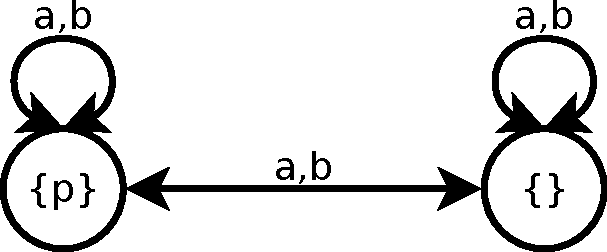
\includegraphics{semantics-coin-s5-1}
}
\caption{\label{semantics-coin-s5-1}
Initially Alice and Bob cannot distinguish between the worlds where the coin
lands on heads or on tails.
}
\end{center}
\end{figure}

Suppose that the coin actually landed on heads. Then the world where $p$ is true
is the actual world. We ask whether it is possible for Alice to learn that the
coin landed on heads whilst Bob continues to be ignorant of the result. We can
represent this question by the following statement in refinement quantified
epistemic logic:
$$\somerefs_a (\knows_a p \land \neg \knows_b p)$$ 

We can show that this statement is satisfied in the actual world of the above
epistemic model, by giving the $a$-refinement in Figure~\ref{semantics-coin-s5-2}

\begin{figure}
\begin{center} 
\scalebox{0.4}{
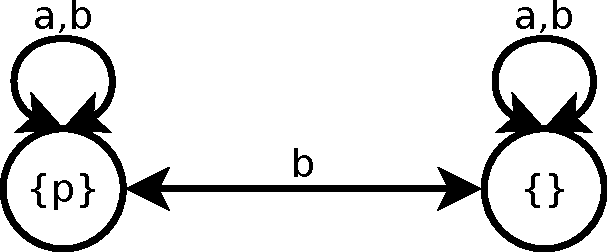
\includegraphics{semantics-coin-s5-2}
}
\caption{\label{semantics-coin-s5-2}
After Alice looks at the coin, she can distinguish between the worlds where the
coin lands on heads or tails, but Bob still cannot.
}
\end{center}
\end{figure}
\end{example}

\begin{example}\label{semantics-coin-kd45}
We recall the coin-flipping example again, but this time in the setting of
doxastic logic. We ask whether it is possible for Alice to come to believe that
the coin landed on heads whilst Bob continues to believe that Alice is ignorant
of the result. We can represent this question by the following statement in
refinement quantified doxastic logic:
$$\somerefs_a (\knows_a p \land \knows_b (\neg \knows_a p \land \neg \knows_a
\neg p))$$

We can show that this statement is satisfied by the model given in
Figure~\ref{semantics-coin-s5-1} by giving the $a$-refinement of the
model in Figure~\ref{semantics-coin-kd45-1}.

\begin{figure}
\begin{center} 
\scalebox{0.4}{
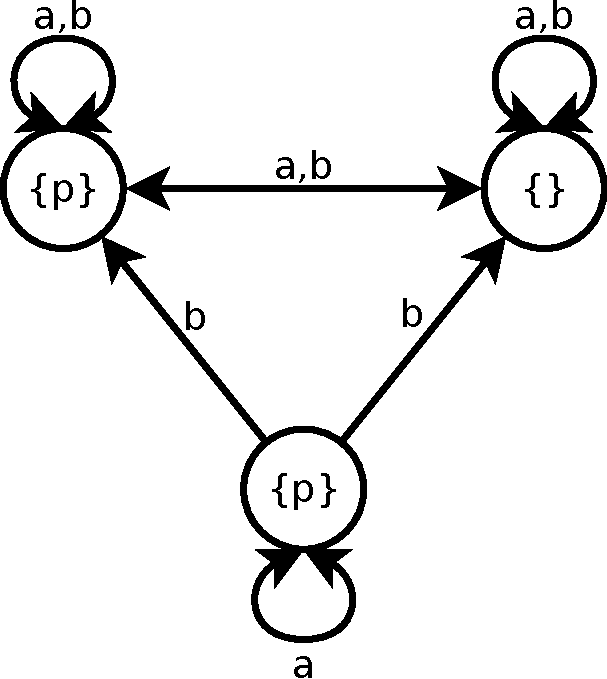
\includegraphics{semantics-coin-kd45}
}
\caption{\label{semantics-coin-kd45-1}
After Alice looks at the coin, she can distinguish between the worlds where the
coin lands on heads or tails, but Bob still cannot distinguish between these
worlds, and neither does he know that Alice can. The actual world is the world
on the bottom.
}
\end{center}
\end{figure}

We note that the statement is not satisfied in the setting of epistemic logic.
This should be clear, as in an epistemic setting, if Alice knows that the coin
landed on heads, then Bob cannot know that this isn't the case, because in an
epistemic setting agents can only know statements that are actually true.
\end{example}

We briefly list some properties of the refinement quantified modal logic, to
give some intuition about the logic. 

\begin{proposition}
We have the following validities: 
\begin{enumerate}
\item $\entails_{\logicKF} \allrefs_a (\phi \implies \psi) \implies \allrefs_a
\phi \implies \allrefs_a \psi$
\item $\entails_{\logicKF} \allrefs_a \phi \implies \phi$
\item $\entails_{\logicKF} \allrefs_a \phi \implies \allrefs_a \allrefs_a \phi$
\item $\entails_{\logicKF} \phi$ implies $\entails_{\logicKF} \allrefs_a \phi$
\item $\entails_{\logicKF} \knows_a \allrefs_a \phi \implies \allrefs_a \knows_a
\phi$
\end{enumerate}
\end{proposition}

These properties were shown by van Ditmarsch and
French~\cite{french2009simulation}. We note that these properties are also valid
in \logicSF{} and \logicKDF{}.

In previous work, van Ditmarsch, French and Pinchinat~\cite{french2010future}
have considered the refinement quantified modal logic, \logicKF{}, based in the
class of models \classK{}. They provided a sound and complete axiomatisation for
the single-agent case, showed that it was expressively equivalent to the
single-agent modal logic, gave a decision procedure for the single-agent case
that runs in 2EXP time, and showed that the refinement quantified modal logic is
exponentially more succinct than the refinement quantified modal logic.

In this thesis we move towards other variants of refinement quantified modal
logics, including the single-agent refinement quantified epistemic and doxastic
logics, and the multi-agent refinement quantified modal and doxastic logics. We
provide sound and complete axiomatisations for each of these logics, and show
that they are expressively equivalent to the modal logics that they are based
on. The expressivity result in particular allows us to show several results for
each of these logics, particularly that they are all decidable.

\chapter{Refinement quantified modal logic}\label{k}

In this chapter we will provide a sound and complete axiomatisation of the
multi-agent refinement quantified modal logic, over the class of \classK{}. 

\section{Technical preliminaries}

In previous work, van Ditmarsch, French and Pinchinat~\cite{french2010future}
gave an axiomatisation of the single-agent variant of the refinement quantified
modal logic \logicKF{}.  The axiomatisation was formulated in terms of the cover
operator, $\covers$, an abbreviation which we defined previously. The
completeness proof consisted of a provably correct translation of formulae from
refinement quantified modal logic to basic modal logic, a translation which
relied on a disjunctive normal form, using the cover operator. Our
axiomatisation for the multi-agent refinement quantified modal logic relies on
the same disjunctive normal form, which we will define now.

\begin{definition}[Disjunctive normal form]
A formula in disjunctive normal form is defined by the following abstract syntax:
$$
\alpha ::= \pi \land \bigwedge_{a \in B} \covers_a \Gamma_a \bnfalt \alpha \lor \alpha
$$
where $\pi$ stands for a propositional formula, $B \subseteq A$, and for $a \in
B$, $\Gamma_a$ stands for a finite set of formulae in disjunctive normal form.
\end{definition}

To show that every \lang{} formula is equivalent to a disjunctive normal
formula, we first introduce the negation normal form and a corresponding lemma
for that form.

\begin{definition}[Negation normal form]
A formula in negation normal form is defined by the following abstract syntax:
$$
\alpha ::= p \bnfalt 
\neg p \bnfalt
\alpha \land \alpha \bnfalt
\alpha \lor \alpha \bnfalt
\knows_a \alpha \bnfalt
\suspects_a \alpha
$$
where $p \in P$ and $a \in A$.
\end{definition}

\begin{lemma}\label{k-nnf}
Every formula of \lang{} is equivalent to a formula in negation normal form,
under the semantics of \logicK{}.
\end{lemma}

\begin{proof}
Similar to negation normal forms in propositional logic, we can recursively push
the negations inwards using the following equivalences:
\begin{eqnarray*}
\neg \neg \phi &\iff& \phi\\
\neg (\phi \land \psi) &\iff& \neg \phi \lor \neg \psi\\
\neg \knows_a \phi &\iff& \suspects_a \neg \phi
\end{eqnarray*}
\end{proof}

\begin{lemma}\label{k-dnf}
Every formula of \lang{} is equivalent to a formula in disjunctive normal form,
under the semantics of \logicK{}.
\end{lemma}

\begin{proof}
Let $\alpha \in \lang$. Without loss of generality, by Lemma~\ref{k-nnf}, we may
assume that $\alpha$ is in negation normal form. We prove by induction over the
structure of $\alpha$ that $\alpha$ is equivalent to a formula in disjunctive
normal form. The induction hypothesis is that every strict subformula of
$\alpha$ has an equivalent in disjunctive normal form.

The base case is when $\alpha = p$ or $\alpha = \neg p$ for some $p \in P$, in
which case we are done.

Suppose that $\alpha = \phi \lor \psi$. By the induction hypothesis, there are
formulae $\phi'$ and $\psi'$ in disjunctive normal form that are equivalent to
$\phi$ and $\psi$ respectively. Then $\phi \lor \psi \iff \phi' \lor \psi'$,
which is in disjunctive normal form.

Suppose that $\alpha = \knows_a \phi$. By the induction hypothesis, there is a
formula $\phi'$ in disjunctive normal form that is equivalent to $\phi$. Then
$\knows_a \phi \iff \covers_a \{\phi\} \lor \covers_a \emptyset$, which is in
disjunctive normal form.

Suppose that $\alpha = \suspects_a \phi$. By the induction hypothesis, there is
a formula $\phi'$ in disjunctive normal form that is equivalent to $\phi$. Then
$\suspects_a \phi \iff \covers_a \{\phi, \top\}$, which is in disjunctive normal
form.

Suppose that $\alpha = \phi \land \psi$. By the induction hypothesis, there are
formulae $\phi'$ and $\psi'$ in disjunctive normal form that are equivalent to
$\phi$ and $\psi$ respectively. Then $\phi \land \psi \iff \phi' \land \psi'$.
As $\phi'$ and $\psi'$ are in disjunctive normal form, then $\phi' = \delta_1
\lor \cdots \lor \delta_m$ and $\psi' = \gamma_1 \lor \cdots \lor \gamma_m$ for
some $m, n \geq 0$, where each of the $\delta_i$ and $\gamma_i$ are terms of the
form $\pi \land \bigwedge_{a \in B \subseteq A} \covers_a \Gamma_a$.  Then we
can rewrite $\alpha$ as a disjunction of conjunctions, by the following
equivalence:
$$
\phi' \land \psi' \iff \bigvee_{i \leq m, j \leq n} \delta_i \land \gamma_j
$$

For each $i \leq m$ and $j \leq n$, we have that $\delta_i = \pi \land
\bigwedge_{a \in B \subseteq A} \covers_a \Gamma_a$, and $\gamma_j = \rho \land
\bigwedge_{a \in C \subseteq A} \covers_a \Gamma'_a$, where $\pi$ and $\rho$ are
propositional formulae, and each $\Gamma_a$ and $\Gamma'_a$ is a set of
disjunctive normal formulae. Then we can write each conjunction as: 
$$\delta_i \land \gamma_i \iff (\pi \land \rho) \land \bigwedge_{a \in B
\subseteq A} \covers_a \Gamma_a \land \bigwedge_{a \in C \subseteq A} \covers_a
\Gamma'_a$$

We note that the sets of agents $B$ and $C$ may intersect, and hence the same
agent may appear in each of those sets, possibly with different sets of formulae
$\Gamma_a$ and $\Gamma'_a$. We can combine the two sets of formulae into one, so
that each agent appears only once, using the following equivalence:
$$
\covers_a \Gamma \land \covers_a \Gamma' \equiv 
\covers_a \big( 
\{ \gamma \land \bigvee_{\gamma' \in \Gamma'} \gamma' \mid \gamma \in \Gamma \}
\cup
\{ \gamma' \land \bigvee_{\gamma \in \Gamma} \gamma \mid \gamma' \in \Gamma' \}
\big)
$$
We note that as each $\gamma \in \Gamma$ and $\gamma' \in \Gamma'$ are assumed
to be disjunctive normal formulae, that applying a disjunction over each of
these sets yields a disjunctive normal formula. Conjoining two disjunctive
normal formulae does not yield a disjunctive normal formula, however an
inductive argument can be used to show that recursively applying the same
translation described here, to each of these conjunctions, yields a disjunctive
normal formula.

Repeating this for each disjunct in our original formula leaves us with a
formula in cover logic disjunctive normal form.

Therefore every formula of \lang{} is equivalent to a formula in disjunctive
normal form.
\end{proof}

We note that, similar to disjunctive normal forms in propositional logic, the
translation into disjunctive normal form in modal logic results in a formula
that is exponentially larger than the original formula in the worst case.

\section{Axiomatisation}

We provide an axiomatisation of the multi-agent refinement quantified modal
logic, \logicKF{}, and prove its soundness and completeness.

\begin{definition}[Axiomatisation \axiomKF]
The axiomatisation \axiomKF{} is a substitution schema consisting of the
following axioms:
$$
\begin{array}{rl}
{\bf P} & \text{All propositional tautologies}\\
{\bf K} & \knows (\phi \implies \psi) \implies \knows \phi \implies \knows
\psi\\
{\bf R} & \allrefs_a (\phi \implies \psi) \implies \allrefs_a \phi \implies
\allrefs_a \psi\\
{\bf RP} & \allrefs_a \alpha \iff \alpha \text{ where $\alpha$ is a
propositional formula}\\
{\bf RComm} & \somerefs_a \covers_b \Gamma \iff \covers_b \{\somerefs_a \gamma
\mid \gamma \in \Gamma\} \text{ where $a \neq b$}\\
{\bf RDist} & \bigwedge_{b \in B} \somerefs_a \covers_b \Gamma_b \implies
\somerefs_a \bigwedge_{b \in B} \covers_b \Gamma_b \text{ where $B \subseteq A$}\\
{\bf RK} & \somerefs_a \covers_a \Gamma \iff \bigwedge_{\gamma \in \Gamma}
\suspects_a \somerefs_a \gamma\\
\end{array}
$$

Along with the rules:
$$
\begin{array}{rl}
{\bf MP} & \text{From $\proves \phi \implies \psi$ and $\proves \phi$, infer
$\proves \psi$}\\
{\bf NecK} & \text{From $\proves \phi$ infer $\proves \knows_a \phi$}\\
{\bf NecR} & \text{From $\proves \phi$ infer $\proves \allrefs_a \phi$}
\end{array}
$$
\end{definition}

% TODO - compare to single-agent axiomatisation
The axiomatisation \axiomKF{} shares many of the axioms and rules of the
axiomatisation from the single-agent case. The axioms {\bf P}, {\bf K}, {\bf R},
{\bf RP} and {\bf RK}, and the rules {\bf MP}, {\bf NecK} and {\bf NecR} are
essentially the same as the axioms that van Ditmarsch, French and
Pinchinat~\cite{french2010future} used in the single-agent case. The differences
are that \axiomKF{} contains axioms for handling the interaction between
multiple agents. The axioms {\bf RComm} and {\bf RDist} are novel axioms used to
handle the situation where a refinement quantifier is applied to a cover
operator of a different agent, and where a refinement quantifier is applied to a
conjunction of cover operators belonging to different agents.

We will now show that the axiomatisation is sound with respect to \classK{}
models.

\begin{lemma}\label{k-sound}
The axiomatisation \axiomKF{} is sound for the class of \classK{} models.
\end{lemma}

\begin{proof}
The soundness of the axioms {\bf P} and {\bf K}, and the rules {\bf MP} and
{\bf NecK} can be shown by the same reasoning used to show that they are sound
in basic modal logic. As the axioms {\bf RP} and {\bf R}, and the rule {\bf
NecR} involve only a single agent, their soundness can be shown by the same
reasoning used to show that they are sound in the single-agent refinement
quantified modal logic~\cite{french2010future}.

All that remains to be shown is the soundness of {\bf RK}, {\bf RComm}, and {\bf
RDist}.

\paragraph{RK}
Suppose that $M_s \in \classK$ is a Kripke model such that $M_s \entails
\bigwedge_{\gamma \in \Gamma} \suspects_a \somerefs_a \gamma$.

We need to show that $M_s \entails \somerefs_a \covers_a \Gamma$. To do this we
will construct a model $N_t \in \classK$, construct an $a$-simulation from $N_t$
to $M_s$ to show that $N_t \refinement_a M_s$, and finally show that $N_t
\entails \covers_a \Gamma$.

We begin by constructing the model $N_t$. Consider $\gamma \in \Gamma$. From
$M_s \entails \suspects_a \somerefs_a \gamma$, there exists a state $s^\gamma
\in sR^M$ such that $M_{s^\gamma} \entails \somerefs_a \gamma$. Therefore there
exists a Kripke model $N^\gamma_{t^\gamma} \refinement_a M_{s^\gamma}$, via some
$a$-simulation $\mathcal{R}^\gamma$, such that $N^\gamma_{t^\gamma} \entails
\gamma$. Without loss of generality we assume that the $N^\gamma$ are disjoint.

Let $t$ be a state not in $S^M$ or any of the $S^{N^\gamma}$. Then we construct a
Kripke model $N = (S^N, R^N, V^N)$ where:
\begin{eqnarray*}
S^N &=& \{t\} \cup S^M \cup \bigcup_{\gamma \in \Gamma} S^{N^\gamma}\\
R^N_a &=& \{(t, t^\gamma) \mid \gamma \in \Gamma\}
\cup R^M_a
\cup \bigcup_{\gamma \in \Gamma} R^{N^\gamma}_a\\
R^N_b &=& \{(t, t') \mid t' \in sR^M_b\}
\cup R^M_b
\cup \bigcup_{\gamma \in \Gamma} R^{N^\gamma}_b \text{ for $b \in A - \{a\}$}\\
V^N(p) &=& 
\begin{cases}
\displaystyle \{t\} \cup V^M(p) \cup \bigcup_{\gamma \in \Gamma} V^{N^\gamma}(p) & \text{if $s
\in V^M(p)$}\\
\displaystyle V^M(p) \cup \bigcup_{\gamma \in \Gamma} V^{N^\gamma}(p) & \text{otherwise}
\end{cases}
\text{ for $p \in P$}
\end{eqnarray*}

\begin{figure}
\begin{center} % TODO - better diagram
\scalebox{0.4}{
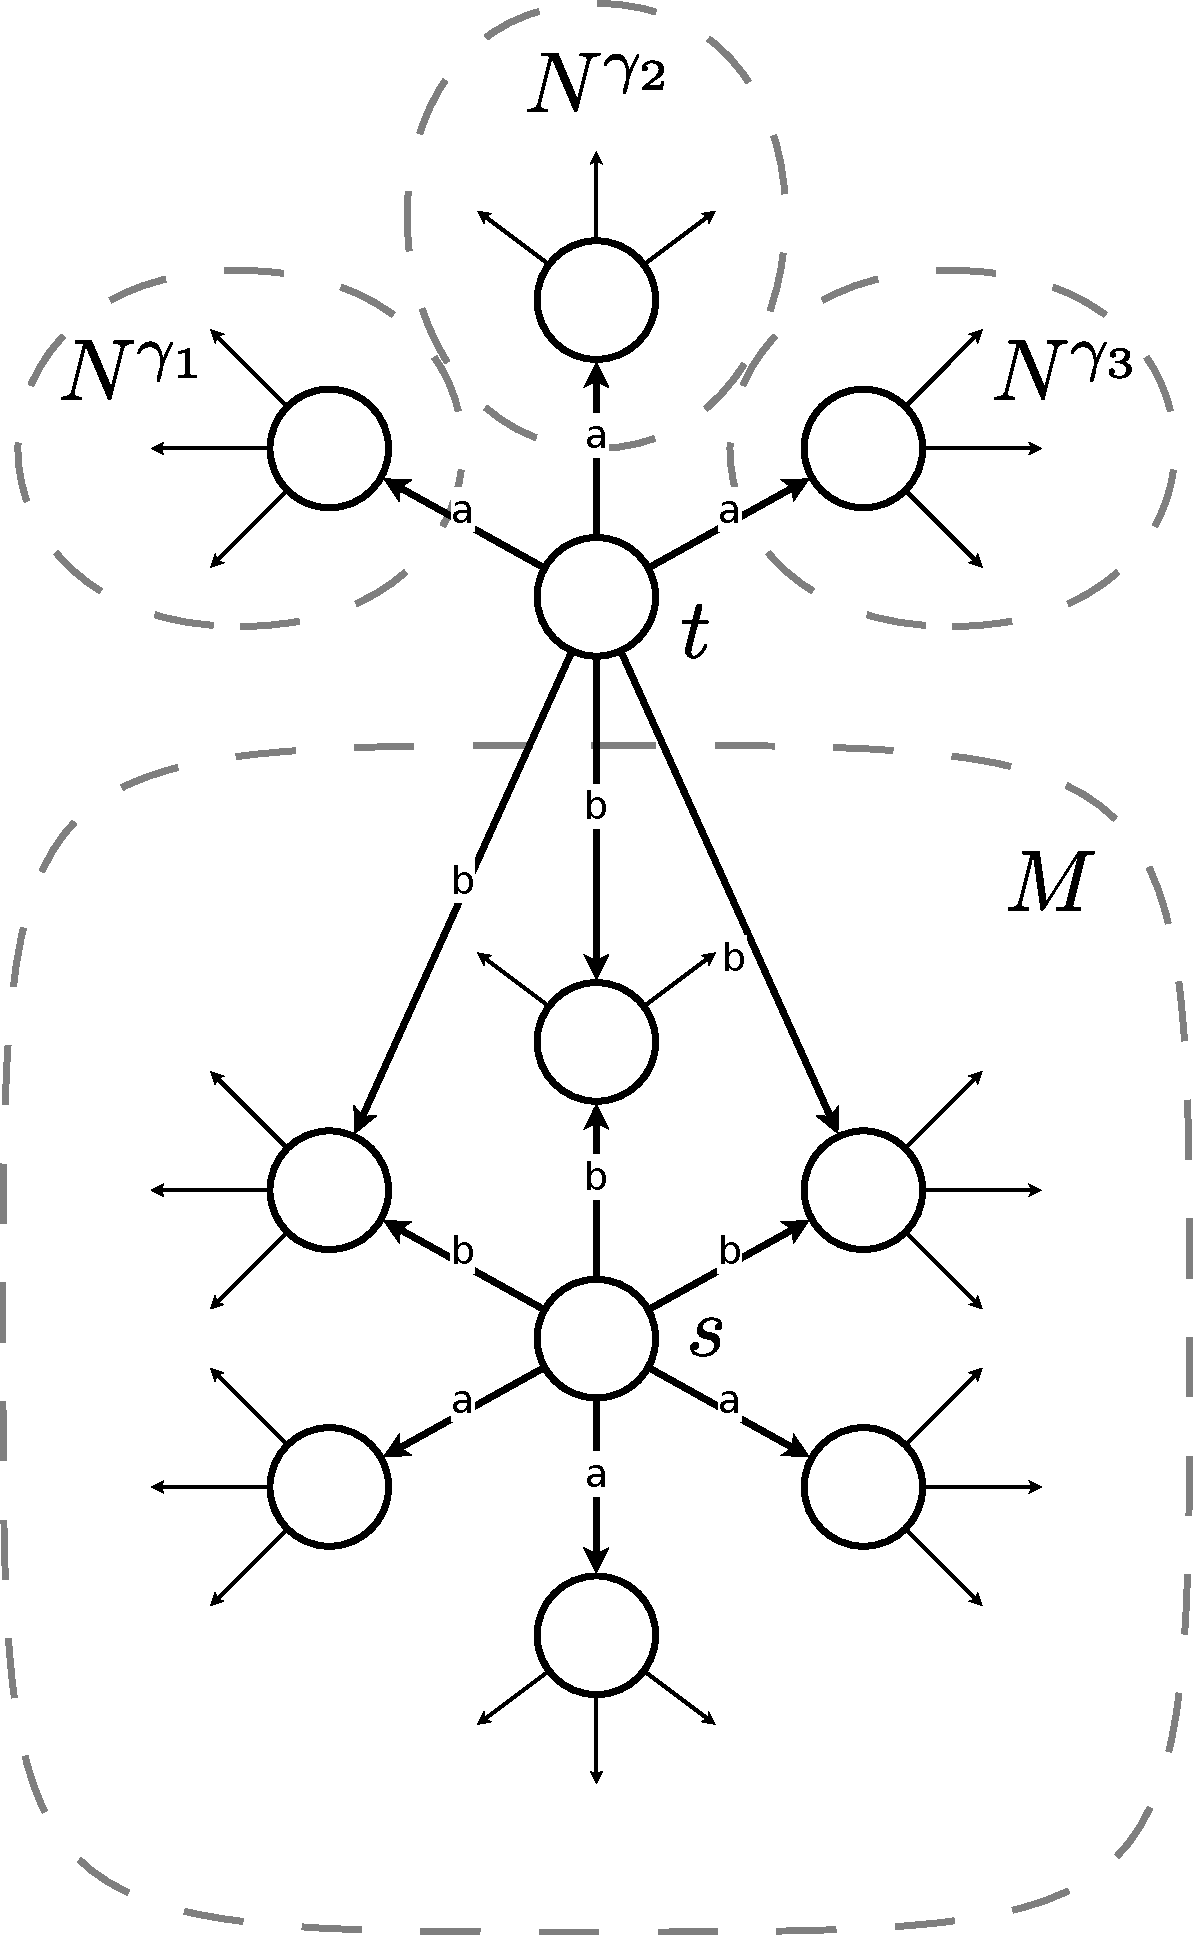
\includegraphics{rk}
}
\caption{
The model $N$ is constructed by taking the model $M$ and the models $N^\gamma$
for every $\gamma \in \Gamma$, and connecting them with an extra node $t$. $t$
is connected via an $a$-edge to $t^\gamma$ from each of the $N^\gamma$, and is
also connected via a $b$-edge to each $b$-successor of $s$ in $M$.
}
\end{center}
\end{figure}

We construct an $a$-simulation $\mathcal{R}$ from $N_t$ to $M_s$, where:
$$\mathcal{R} = \{(t, s)\} \cup \{(s', s') \mid s' \in S^M \} 
\cup \bigcup_{\gamma \in \Gamma} \mathcal{R}^\gamma$$

We must show that $\mathcal{R}$ satisfies {\bf atoms}, {\bf forth-$b$} for every
$b \in A$, and {\bf back-$b$} for every $b \in A - \{a\}$.

\paragraph{atoms} We note that, by construction, the valuation of $N$ matches
the valuation of its corresponding states in $M$ and each $N^\gamma$, and the
valuation of $N_t$ matches that of $M_s$. Therefore $\mathcal{R}$ satisfies {\bf
atoms}.

\paragraph{forth} We next show that $\mathcal{R}$ satisfies {\bf forth-$b$} for
every $b \in A$.  Let $b \in A$ and let $(u, v) \in \mathcal{R}$.

Suppose that $(u, v) \in \mathcal{R}^\gamma$ for some $\gamma \in \Gamma$.  Then
as $\mathcal{R}^\gamma$ is an $a$-simulation, it satisfies {\bf forth-$b$} for
every $b \in A$. Hence for every $u' \in uR^{N^\gamma}_b = uR^N_b$, there exists
some $v' \in vR^M_b$ such that $(u', v') \in \mathcal{R}^\gamma \subseteq
\mathcal{R}$. 

Suppose instead that $(u, v) = (s', s')$ for some $s' \in S^M$.  Then we note
that $s'R^N_b = s'R^M_b$, and hence for every $s'' \in s'R^N_b$ we have that
$s'' \in s'R^M_b$, and that $(s'', s'') \in \mathcal{R}$. 

Finally suppose that $(u, u') = (t, s)$. We must consider the cases where $b =
a$ and where $b \neq a$. So suppose that $b = a$. By construction, $tR^N_a =
\{t^\gamma \mid \gamma \in \Gamma\}$, and hence $v = t^\gamma$ for some $\gamma
\in \Gamma$. Hence we can take $s^\gamma \in sR^M_a$, and note that as
$\mathcal{R}^\gamma$ is an $a$-simulation from $M_{s^\gamma}$ to
$N^\gamma_{t^\gamma}$, we know that $(t^\gamma, s^\gamma) \in \mathcal{R}^\gamma
\subseteq \mathcal{R}$. Suppose that $b \neq a$. Then by construction, $tR^M_b =
sR^M_b$, hence for every $t' \in tR^M_b$, we have that $t' \in sR^M_b$, and
hence we know that $(t', t') \in \mathcal{R}$. 

Therefore $\mathcal{R}$ satisfies {\bf forth-$b$} for every $b \in A$.

\paragraph{back} A similar argument to above shows that $\mathcal{R}$
satisfies {\bf back-$a$} for every $b \in A - \{a\}$.

Therefore $\mathcal{R}$ is an $a$-simulation, and $N_t \refinement_a M_s$.

Finally we show that $N_t \entails \covers_a \Gamma$. We must show that for each
$\gamma \in \Gamma$ that $N_{t^\gamma} \entails \gamma$. This follows from the
fact that $N_{t^\gamma}$ is bisimilar to $N^\gamma_{t^\gamma}$. This is obvious,
as $N$ contains a duplicate of $N^\gamma$, and $N$ does not add any additional
edges originating from states in $S^{N^\gamma}$. Hence from bisimulation
invariance, $N_{t^\gamma} \entails \gamma$ for every $\gamma \in \Gamma$, and
hence $N_t \entails \covers_a \Gamma$.

As $N_t \refinement_a M_s$, and $N_t \entails \covers_a \Gamma$ we therefore
have that $M_s \entails \somerefs_a \covers_a \Gamma$.

Conversely, suppose that $M_s \entails \covers_a \Gamma$. Then there exists a
Kripke model $N_t \refinement_a M_s$, via some $a$-simulation $\mathcal{R}$,
such that $N_t \entails \covers_a \Gamma$. From the definition of the cover
operator, this implies that $N_t \entails \knows_a \bigvee_{\gamma \in \Gamma}
\gamma \land \bigwedge_{\gamma \in \Gamma} \suspects_a \gamma$. In particular we
note that for every $\gamma \in \Gamma$, $N_t \entails \suspects_a \gamma$, and
so there exists some $t^\gamma \in tR^N_a$ such that $N_{t^\gamma} \entails
\gamma$. As $t^\gamma \in tR^N_a$, and $(t, s) \in \mathcal{R}$, by {\bf
forth-$a$} there exists some $s^\gamma \in sR^M_a$ such that $(t^\gamma, s^\gamma)
\in \mathcal{R}$. Hence $\mathcal{R}$ is also an $a$-simulation from
$N_{t^\gamma}$ to $M_{s^\gamma}$, and so $M_{s^\gamma} \entails \somerefs_a
\gamma$. As for every $\gamma \in \Gamma$ we have that $s^\gamma \in sR^M_a$, we
also have that $M_s \entails \suspects_a \somerefs_a \gamma$. Therefore we
finally have that $M_s \entails \bigwedge_{\gamma \in \Gamma} \suspects_a
\somerefs_a \gamma$.

Therefore {\bf RK} is sound.

\paragraph{RComm}
Suppose that $M_s \in \classK$ is a Kripke model such that $M_s \entails
\covers_b \{ \somerefs_a \gamma \mid \gamma \in \Gamma\}$, where $a \neq b$.

We need to show that $M_s \entails \somerefs_a \covers_b \Gamma$. To do this we
follow the same strategy as for proving {\bf RK}: we construct an $a$-refinement
$N_t \in \classK$, and show that $N_t \entails \covers_b \Gamma$.

We begin by constructing the model $N_t$. Consider $\gamma \in \Gamma$. From
$M_s \entails \covers_b \{ \somerefs_a \gamma \mid \gamma \in \Gamma \}$, there
exists a state $s^\gamma \in sR^M_b$ such that $M_{s^\gamma} \entails
\somerefs_a \gamma$. Therefore there exists a Kripke model $N^\gamma_{t^\gamma}
\refinement_a M_{s^\gamma}$, via some $a$-simulation $\mathcal{R}^\gamma$, such
that $N^\gamma_{t^\gamma} \entails \gamma$. Without loss of generality we assume
that the $N^\gamma$ are disjoint.

Let $t$ be a state not in $S^M$ or any of the $S^{N^\gamma}$. Then we construct a
Kripke model $N = (S^N, R^N, V^N)$ where:
\begin{eqnarray*}
S^N &=& \{t\} \cup S^M \bigcup_{\gamma \in \Gamma} S^{N^\gamma}\\
R^N_b &=& \{(t, t^\gamma) \mid \gamma \in \Gamma\} 
\cup  R^M_b 
\cup \bigcup_{\gamma \in \Gamma} R^{N^\gamma}_b\\
R^N_c &=& \{(t, t') \mid t' \in sR^M_c\} 
\cup R^M_c \cup \bigcup_{\gamma \in \Gamma} R^{N^\gamma}_c \text{ for $c \in A - \{b\}$}\\
V^N(p) &=& 
\begin{cases}
\displaystyle \{t\} \cup V^M(p) \cup \bigcup_{\gamma \in \Gamma} V^{N^\gamma}(p)
& \text{if $s \in V^M(p)$}\\
\displaystyle V^M(p) \cup \bigcup_{\gamma \in \Gamma} V^{N^\gamma}(p) &
\text{otherwise}
\end{cases}
\text{ for $p \in P$}
\end{eqnarray*}

We construct an $a$-simulation $\mathcal{R}$ from $N_t$ to $M_s$, where:
$$\mathcal{R} = \{(t, s)\} \cup \{(s', s') \mid s' \in S^M\} \cup
\bigcup_{\gamma \in \Gamma} \mathcal{R}^\gamma$$

We note that $\mathcal{R}$ is an $a$-simulation, by similar arguments as used in
the proof for {\bf RK}. In particular, this means that $N_t \refinement_a M_s$.

We also note that for every $\gamma \in \Gamma$, that $N_{t^\gamma} \entails
\gamma$, by similar arguments as used in the proof for {\bf RK}. In particular,
this means that $N^\gamma_t \entails \covers_b \Gamma$.

Therefore $M_s \entails \somerefs_a \covers_b \Gamma$.

The converse, $\somerefs_a \covers_b \Gamma \implies \covers_b \{\somerefs_a
\gamma \mid \gamma \in \Gamma\}$ follows a similar proof to the relevant part in
the proof for {\bf RK}.

Therefore {\bf RComm} is sound.

\paragraph{RDist}
Suppose that $M_s \in \classK$ is a Kripke model such that $M_s \entails
\bigwedge_{b \in B} \somerefs_a \covers_b \Gamma_b$, where $B \subseteq A$.

We need to show that $M_s \entails \somerefs_a \bigwedge_{b \in B} \covers_b
\Gamma_b$. To do this we follow the same strategy as for proving {\bf RK}: we
construct an $a$-refinement $N_t \in \classK$, and show that $N_t \entails
\somerefs_a \bigwedge_{b \in B} \covers_b \Gamma_b$.

We begin by constructing the model $N_t$. Suppose that $a \in B$. Then we have
$M_s \entails \somerefs_a \covers_a \Gamma_a$, and by {\bf RK} this implies that
$M_s \entails \bigwedge_{\gamma \in \Gamma_a} \gamma$. We also have that for
every $b \in B - \{a\}$ that $M_s \entails \somerefs_a \covers_a \Gamma_b$, and
by {\bf RComm} this implies that $M_s \entails \covers_b \{\somerefs_a \gamma
\mid \gamma \in \Gamma_b\}$, and by the definition of the cover operator, this
implies that $M_s \entails \bigwedge_{\gamma \in \Gamma_b} \suspects_b
\somerefs_a \gamma$. Hence for every $b \in B$ and $\gamma \in \Gamma_b$, we
have that $\suspects_b \somerefs_a \gamma$. This implies that for each $b \in B$
and each $\gamma \in \Gamma_b$ that there exists some $s^{b,\gamma} \in sR^M_b$ such
that $M_{s^{a,\gamma}} \entails \somerefs_a \gamma$. Therefore there exists a Kripke
model $N^{b,\gamma}_{t^{b,\gamma}} \refinement_a M_{s^{a,\gamma}}$ such that
$N^{b,\gamma}_{t^{b,\gamma}} \entails \gamma$. Without loss of generality we
may assume that the $N^{b,\gamma}$ are disjoint.

Let $t$ be a state not in $S^M$ or any of the $S^{N^{b,\gamma}}$. Then we construct a
Kripke model $N = (S^N, R^N, V^N)$ where:
\begin{eqnarray*}
S^N &=& \{t\} \cup S^M \cup \bigcup_{b \in A, \gamma \in \Gamma_b} S^{N^{b,\gamma}}\\
R^N_b &=& \{(t, t^{b,\gamma}) \mid \gamma \in \Gamma_b\} \cup R^M_b \cup
\bigcup_{c \in B, \gamma \in \Gamma_c} R^{N^{c,\gamma}}_b \text{ for $b \in
B$}\\
R^N_b &=& \{(t, t') \mid t' \in sR^M_b\} \cup R^M_b \cup
\bigcup_{c \in B, \gamma \in \Gamma_c} R^{N^{c,\gamma}}_b \text{ for $b \in A
\setminus B$}\\
V^N(p) &=& 
\begin{cases}
\displaystyle \{t\} \cup V^M(p) \cup \bigcup_{b \in B, \gamma \in \Gamma_b}
V^{N^{b,\gamma}}(p) & \text{if $s \in V^M(p)$}\\
\displaystyle V^M(p) \cup \bigcup_{b \in B, \gamma \in \Gamma_b}
V^{N^{b,\gamma}}(p) & \text{otherwise}
\end{cases}
\end{eqnarray*}

We construct an $a$-simulation $\mathcal{R}$ from $N_t$ to $M_s$, where:
$$\mathcal{R} = \{(t, s)\} \cup \{(s', s') \mid s' \in S^M\} \bigcup_{b \in A,
\gamma \in \Gamma_b} \mathcal{R}^\gamma$$

We note that this is an $a$-simulation, by similar arguments as used in the
proof for {\bf RK}. In particular, this means that $N_t \refinement_a M_s$.

We also note that for every $b \in A$, and $\gamma \in \Gamma_b$ that
$N_{t^\gamma} \bisim N^\gamma_{t^\gamma}$, by similar arguments as used in the
proof for {\bf RK}. In particular, this means that as $N^\gamma_{t^\gamma}
\entails \gamma$ that we also have $N_{t^\gamma} \entails \gamma$, for every $b
\in A$ and $\gamma \in \Gamma_b$. Therefore $N_t \entails \covers_b \Gamma_b$
for every $b \in A$, and therefore $N_t \entails \bigwedge_{b \in A} \covers_b
\Gamma_b$.

Therefore $M_s \entails \somerefs_a \bigwedge_{b \in A} \covers_b \Gamma_b$ and
{\bf RDist} is sound.

Therefore the axiomatisation \axiomKF{} is sound.
\end{proof}

We note that if the implication in {\bf RDist} is strengthened to an equality,
that the resulting axiom is also sound. However this is easily derivable from
the other axioms in \axiomKF{}.

\begin{lemma}\label{k-rdist-converse}
The following is derivable in \axiomKF{}.
$$
\proves \bigwedge_{b \in A} \somerefs_a \covers_b \Gamma_b \iff
\somerefs_a \bigwedge_{b \in A} \covers_b \Gamma_b \\
$$
where $\Gamma_b$ is a set of $b$-disjunctive normal formulae for
every $b \in A$.
\end{lemma}

\begin{proof}[Proof (Sketch)]
The forward direction is the axiom {\bf RDist}. 

The converse can be derived in a more general form as $\somerefs_a (\phi \land
\psi) \implies \somerefs_a \phi \land \somerefs_a \psi$. The derivation is
similar to the derivation for $\knows_a (\phi \land \psi) \implies \knows_a \phi
\land \knows_a \psi$ in the modal logic \logicK{}, using the axiom {\bf R} in
place of {\bf K}.
\end{proof}

We show the completeness of the axiomatisation \axiomKF{} by a provably correct
translation from \langF{} to \lang{}. Completeness then follows from the
completeness of \logicK{}.

We introduce some equivalences that will be used by our translation.

\begin{lemma}\label{k-equivalences}
The following are provable equivalences using \axiomKF{}:
\begin{enumerate}
\item $\displaystyle \somerefs_a (\phi \lor \psi) \iff
\somerefs_a \phi \lor \somerefs_a \psi$
\item $\displaystyle \somerefs_a (\pi \land \bigwedge_{b
\in B} \covers_b \Gamma_b) \iff \pi \land \bigwedge_{\gamma \in \Gamma_a}
\suspects_a \somerefs_a \gamma \land \bigwedge_{b \in B} \covers_b \{\somerefs_a
\gamma \mid \gamma \in \Gamma_b\}$ where $\pi$ is propositional, $B \subseteq
A$, and $a \in B$
\item $\displaystyle \somerefs_a (\pi \land \bigwedge_{b
\in B} \covers_b \Gamma_b) \iff \pi \land \bigwedge_{b \in B} \covers_b
\{\somerefs_a \gamma \mid \gamma \in \Gamma_b\}$ where $\pi$ is propositional,
$B \subseteq A$, and $a \notin B$
\end{enumerate}
\end{lemma}

\begin{proof}
(1) is derivable from {\bf P} and {\bf R} using the same strategy used to prove
that $\suspects_a (\phi \lor \psi) \iff \suspects_a \phi \lor \suspects_a \psi$
is derivable from {\bf P} and {\bf K}.

(2) and (3) are derivable, by using {\bf P}, {\bf R} and {\bf RP} to bring the
propositional part $\pi$ outside the $\somerefs_a$ operator, using {\bf RDist}
zsh:1: command not found: :pdflatex
$\somerefs_a$ operator into the cover operators inside the conjunction, and then
using {\bf RK} or {\bf RComm} as appropriate for each cover operator.
\end{proof}

\begin{lemma}\label{k-translation}
Every formula of \langF{} is provably equivalent to a formula of \lang{} with
the axiomatisation \axiomKF{}.
\end{lemma}

\begin{proof}
Let $\alpha \in \langF{}$. We assume without loss of generality that all
\allrefs{} operators are expressed as \somerefs{} operators, by the equivalence
$\allrefs_a \phi \iff \neg \somerefs_a \neg \phi$. We prove by induction on the
number of occurrences of \somerefs{} in $\alpha$ that $\alpha$ is equivalent to
a \somerefs{}-free formula, and therefore to a formula in \lang{}. The base
case where $\alpha$ contains no \somerefs{} operators is trivial, as a
\somerefs{}-free formula is a formula in \lang{}. Suppose instead that $\alpha$
contains $n + 1$ \somerefs{} operators, and assume that any formula with $n$
\somerefs{} operators is provably equivalent to a formula in \lang{}. We use
the axioms of \axiomKF{} to show that $\alpha$ is provably equivalent to a
formula with $n$ \somerefs{} operators, and that therefore by the induction
hypothesis it is provably equivalent to a formula in \lang{}.

Choose a subformula from $\alpha$ of type $\somerefs_a \beta$, where $\beta$ is
\somerefs{}-free. Without loss of generality, by Lemma~\ref{k-dnf} we may assume
that $\beta$ is in disjunctive normal form. We prove by induction on the
structure of $\beta$ that $\somerefs_a \beta$ is provably equivalent to a
formula $\chi \in \lang$. The induction hypothesis is that for any proper
subformula $\phi$ of $\beta$ that $\somerefs_a \phi$ is equivalent to a formula
in \lang{}.

The base case is when $\beta$ is a propositional formula. In this case, from
{\bf P} and {\bf RP}, we have that $\somerefs_a \beta \iff \beta$, and therefore
$\somerefs_a \beta$ is equivalent to a formula in \lang{}. 

The inductive case is when $\beta = \phi \lor \psi$, or when $\beta = \pi \land
\bigwedge_{b \in B} \covers_b \Gamma_b$, where $B \subseteq A$. We note that we
can use the equivalences from Lemma~\ref{k-equivalences} to push the $\somerefs_a$
operator inside so that it is applied to subformulae of $\beta$. We can then use
the induction hypothesis to replace each occurrence of the $\somerefs_a$
operator applied to a subformula of $\beta$ with an equivalent formula in
\lang{}. The resulting formula is also in \lang{}.

Therefore by the principle of mathematical induction, $\somerefs_a \beta$ is
equivalent to a formula $\chi \in \lang{}$ for every $\beta \in \lang{}$. 

Hence replacing $\somerefs_a \beta$ in $\alpha$ with $\chi$ gives an equivalent
formula that contains only $n$ \somerefs{} operators.

Therefore by the principle of mathematical induction, $\alpha$ is equivalent to
a formula in \lang{}.
\end{proof}

The rest of the completeness proof is merely a formality to show that, given the
above translation into \lang{}, we can show completeness by using these
translations along with the completeness of \logicK{}.

\begin{corollary}\label{k-derivable}
Let $\phi \in \langF$ be given and $\psi \in \lang$ be semantically
equivalent to $\phi$.  If $\psi$ is a theorem in \logicK{}, then $\phi$ is a
theorem in \axiomKF{}.
\end{corollary}

\begin{proof} % TODO - replace with reference to \ref{single-derivable-s5} ?
Let $\phi \in \langF$ and let $\psi \in \lang$ be semantically equivalent to
$\phi$. By Lemma~\ref{k-translation}, we can obtain some $\phi' \in \lang$
that is semantically equivalent to $\phi$ (and thus also to $\psi$) by following
the given translation steps. We can extend a derivation of $\psi$ to a
derivation of $\phi'$ as the two are semantically equivalent in \logicK{}, and by
the completeness of \logicK{} this equivalence is derivable. As \axiomKF{} is a
conservative extension of \logicK{}, this equivalence is therefore also derivable
in \axiomKF{}. The derivation can be further extended to $\phi$ by observing that all
of the reduction steps in Lemma~\ref{k-translation} are provable equivalences
in \axiomKF{}. Therefore $\phi$ is a theorem in \axiomKF{}.
\end{proof}

\begin{lemma}\label{k-complete}
The axiom schema \axiomKF{} is complete for the logic \logicKF{}.
\end{lemma}

\begin{proof}
Let $\phi \in \langF$ such that $\classK \entails_\somerefs \phi$. Then by
Lemma~\ref{k-translation}, there exists a semantically equivalent formula
$\psi \in \lang$ which is \somerefs-free. As $\classK \entails_\somerefs \phi$ and
$\phi \iff \psi$, then $\classK \entails_\somerefs \psi$. As $\psi$ is
\somerefs-free, then it follows that $\classK \entails \psi$, and by the
completeness of \axiomKF{} it follows that $\proves_{\axiomK} \psi$.
Therefore by Corollary~\ref{k-derivable} we have that $\proves_{\axiomKF}
\phi$.
\end{proof}

\begin{theorem}
The axiomatisation \axiomKF{} is sound and complete for the logic \logicKF{}.
\end{theorem}

\begin{proof}
The soundness proof is given in Lemma~\ref{k-sound} and the completeness
proof is given in Lemma~\ref{k-complete}.
\end{proof}

We note that, as in the axiomatisation for the single-agent epistemic and
doxastic logics, the completeness proofs above were performed with a provably
correct translation from \langF{} to \lang{}, under the semantics of
\logicKF{}. This shows that \logicKF{} is expressively equivalent to
\logicK{}, and allows us to show several results. In particular, \logicKF{} is
decidable.

\begin{theorem}
The logic \logicKF{} is decidable.
\end{theorem}

This can be shown by following similar reasoning as used for the proof of
Theorem~\ref{single-decidable}.

\chapter{Doxastic logic}\label{chapter-doxastic}

\section{Syntax and semantics}

Here we define the syntax and semantics of the logic \logicKDF{}, which
restricts the logic \logicKF{}, as defined by van Ditmarsch and
French~\cite{french2009simulation}, to deal with only models and refinements of
doxastic models.

% TODO - more motiviation

\begin{definition}[Language of \langF{}] % TODO - move to the K section
Given a finite set of agents $A$ and a set of propositional atoms $P$, the
language of \langF{} is defined by the following abstract syntax:

$$
\phi ::=    p \bnfalt
            \neg \phi \bnfalt
            \phi \land \phi \bnfalt
            \knows_a \phi \bnfalt
            \allrefs_a \phi
$$
where $a \in A$ and $p \in P$.
\end{definition}

Standard abbreviations include:
$\top ::= \phi \lor \neg \phi$;
$\bot ::= \neg \top$;
$\phi \lor \psi ::= \neg (\neg \phi \land \neg \psi)$;
$\phi \implies \psi ::= \neg \phi \lor \psi$;
and $\suspects_a \phi ::= \neg \knows_a \neg \phi$.
We use an abbreviation for the dual of the $\allrefs_a$ operator,
$\somerefs_a \phi ::= \neg \allrefs_a \neg \phi$.

We also use the cover operator $\covers_a \Gamma$, where $\Gamma$ is a finite
set of formulae, which is an abbreviation for 
$\covers_a \Gamma ::= \knows_a \bigvee_{\gamma \in \Gamma} \gamma \land
\bigwedge_{\gamma \in \Gamma} \suspects_a \gamma$. The cover operator is relied
on for our axiomatisation, in much the same way it is relied on for the
axiomatisation of \logicKiF{} presented by van Ditmarsch, French and
Pinchinat~\cite{french2010future}. % TODO - include citation for cover operator

\begin{definition}[Semantics of \logicKDF{}]
Let $M = (S, R, V)$ be a doxastic model. The interpretation of $\phi \in
\logicKDF$ is defined inductively.

\begin{eqnarray*}
M_s &\entails& p \text{ iff } s \in V_p\\
M_s &\entails& \neg \phi \text{ iff } M_s \nentails \phi\\
M_s &\entails& \phi \land \psi \text{ iff } M_s \entails \phi \text{ and } M_s
\entails \psi\\
M_s &\entails& \knows_a \phi \text{ if for all } t \in S : (s, t) \in R_a \text{
implies } M_t \entails \phi\\
M_s &\entails& \allrefs_a \phi \text{ iff for all } M'_{s'} \in \classKD : M_s
\simulation_a M'_{s'} \text{ implies } M'_{s'} \entails \phi\\
\end{eqnarray*}
\end{definition}

The difference between \logicKF{} and \logicKDF{} is in the class of models that
they are interpreted over. It should be emphasised that the interpretation of
the refinement operator, $\allrefs_a$, varies for each logic, as the refinements
considered in the interpretation of the operator in \logicKDF{} must be taken
from the class of doxastic models, \classKD{}, whereas in \logicKF{} they may be
arbitrary Kripke models from \classK{}. It is for this reason that \logicKDF{}
is not a conservative extension of \logicKF{}. 

For example, the formula $\somerefs_a \knows_a \bot$ is valid in \logicKF{}, as
given any pointed Kripke model $M_s$, one can always form an $a$-refinement
$M'_{s'}$ of $M_s$ which simply removes all $a$-edges from $s$ in $M_s$, so that
$M'_{s'} \entails \knows_a \bot$. However $\somerefs_a \knows_a \bot$ is not
valid in \logicKDF{}, as all doxastic models have the serial property, and
hence there are no models in which $\knows_a \bot$ is true; therefore no
doxastic models can have a refinement where that is true.

\begin{lemma}
The logic \logicKDF{} is bisimulation invariant.
\end{lemma}

The proof for the bisimulation invariance of \logicKF{}, given by van Ditmarsch,
French and Pinchinat~\cite{french2010future} also applies to \logicKDF{}. 
% TODO - more explanation?

% TODO - examples

In previous work we gave an axiomatisation of the single-agent variant of
\logicKDF{}, called \logicKDiF{}, which relied upon a prenex normal form for the
well-formed formulae of \logicKDi{}. The prenex normal form prohibits modal
operators ($\knows$ and $\suspects$) from appearing within other modal
operators, and we showed that all \logicKDi{} formulae are equivalent to a
formula in prenex normal form. The prenex normal form simplified the
axiomatisation and proof of soundness by avoiding complications that would
arise due to the transitivity of doxastic models.

We introduce a disjunctive normal form for the multi-agent logic \logicKD{},
which achieves the same purpose in terms of our axiomatisation as the prenex
normal form did for the single-agent \logicKD{}. In the multi-agent logic, it is
not possible to express all formulae in a form which prohibits nested modal
operators as in the prenex normal form, however it is possible to prohibit the
modal operators belonging to an agent $a$ (i.e. $\knows_a$ and $\suspects_a$)
from appearing directly within the scope of another modal operator belonging to
$a$. This allows us to avoid complications due to transitivity in our proof of
soundness for our axiomatisation of \logicKDF{}, in much the same way that
prenex normal form did for the axiomatisation of \logicKDiF{}.

\begin{definition}[Disjunctive normal form]
A formula in $a$-disjunctive normal form is defined by the following abstract syntax:

\begin{eqnarray*}
\alpha &::=& \delta \bnfalt \alpha \lor \alpha\\
\delta &::=& \pi \bnfalt \knows_b \gamma_b \bnfalt \suspects_b \gamma_b \bnfalt
\delta \land \delta\\
\end{eqnarray*}
where $\pi$ stands for a propositional formula, $b \in A - \{a\}$, and
$\gamma_b$ stands for a formula in $b$-disjunctive normal form.

A formula in disjunctive normal form is defined by the following abstract syntax:

\begin{eqnarray*}
\alpha &::=& \delta \bnfalt \alpha \lor \alpha\\
\delta &::=& \pi \bnfalt \knows_a \gamma_a \bnfalt \suspects_a \gamma_a \bnfalt
\delta \land \delta\\
\end{eqnarray*}
where $\pi$ stands for a propositional formula, $a \in A$, and $\gamma_a$
stands for a formula in $a$-disjunctive normal form.
\end{definition}

\begin{lemma}\label{kd45-dnf-equivalences}
We have the following equivalences in \logicKD{}:

\begin{eqnarray*}
\knows_a (\pi \lor (\alpha \land \knows_a \beta)) &\iff& (\knows_a (\pi \lor \alpha)
\land \knows_a \beta) \lor (\knows_a \pi \land \neg \knows_a \beta)\\
\knows_a (\pi \lor (\alpha \land \suspects_a \beta)) &\iff& (\knows_a (\pi \lor \alpha)
\land \suspects_a \beta) \lor (\knows_a \pi \land \neg \suspects_a \beta)
\end{eqnarray*}
\end{lemma}

This is proven by Meyer and van der Hoek~\cite{meyer2004epistemic} for
\logicSi{}, however the same proof also applies to \logicKD{}.

Meyer and van der Hoek remarked that the only use of the reflexivity axiom of
\logicS{}, {\bf T}, in the proof, is in the form of the theorems $\proves \knows
\knows \phi \implies \knows \phi$, and $\proves \knows \neg \knows \phi \implies
\neg \knows \phi$. Therefore the proof holds for any logic which replaces {\bf
T} with axioms entailing both of these properties. Both of these properties are
obviously valid in \logicKD{}, and therefore the proof by Meyer and van der
Hoek~\cite{meyer2004epistemic} applies to this result.

\begin{lemma}\label{kd45-dnf}
Every well-formed formula of \logicKD{} is equivalent to a formula in
disjunctive normal form.
\end{lemma}

\begin{proof}
We use a proof similar to the proof for prenex normal form, given by Meyer and
van der Hoek~\cite{meyer2004epistemic}.

Let $\phi$ be a well-formed formula of \logicKD{}. We proceed by induction on
the structure of $\phi$, with the induction hypothesis that every strict
subformula of $\phi$ is equivalent to a formula in disjunctive normal form.

Suppose that $\phi$ is a proposition. Then we are done; $\phi$ is in disjunctive
normal form.

Suppose that $\phi = \neg \alpha$. Then by the induction hypothesis, $\alpha$ is
equivalent to some $\alpha'$ in disjunctive normal form. We can use an inductive
argument, over $\alpha'$, to show that De Morgan's law can be repeatedly applied
to $\alpha'$ until the negation is pushed inwards, so that the only negations
are applied to propositional formulae (the result of which is a propositional
formula), thus yielding a formula equivalent to $\phi$. The result of this
process is a formula in disjunctive normal form. % TODO - more detail

Suppose that $\phi = \alpha \land \beta$. Then by the induction hypothesis, $\alpha$
and $\beta$ are equivalent to some $\alpha'$ and $\beta'$ in disjunctive normal
form. We note that we can equivalently write $\phi$ as $\phi = \neg (\neg
\alpha' \lor \neg \beta')$. From our case for negation, we note that $\neg
\alpha'$ and $\neg \beta'$ are equivalent to some $\alpha''$ and $\beta''$ in
disjunctive normal form. Given these, $\alpha'' \lor \beta''$ is also is
disjunctive normal form. Thus we can use our case for negation once again to
note that $\phi = \neg \alpha'' \lor \beta''$ is equivalent to some $\phi''$ in
disjunctive normal form.

Suppose that $\phi = \knows_a \psi$. Then by the induction hypothesis, $\psi$ is
equivalent to some $\psi'$ in disjunctive normal form. Suppose that $\psi'$ is
not in $a$-disjunctive normal form (otherwise we are done). Then $\psi'$
contains some conjunct of the form $\knows_a \beta$ or $\suspects_a \beta$. Thus
we can rewrite $\psi'$ as $\psi' = \pi \lor (\alpha \land \knows_a \beta)$. By
Lemma \ref{kd45-dnf-equivalences}, we get that $\phi \equiv (\knows_a (\pi \lor
\alpha) \land \knows_a \beta) \lor (\knows_a \pi \land \neg \knows_a \beta)$. We
can use the other equivalence from Lemma \ref{kd45-dnf-equivalences} in the case
that $\phi = \suspects_a \psi$.

Proceeding in this fashion we may move all conjuncts of $\psi'$ containing an
$a$-modality to the outside, so that they are conjuncts of $\phi$, thus
obtaining a formula in disjunctive normal form. % TODO - Make clearer
\end{proof}

\begin{definition}[Cover disjunctive normal form]\label{kd45-cdnf}
A formula in $a$-cover disjunctive normal form is defined by the following
abstract syntax:

$$
\alpha ::= \pi \land \bigwedge_{b \in A - \{a\}} \covers_b \Gamma_b \bnfalt
\alpha \lor \alpha
$$
where $\pi$ stands for a propositional formula, and $\Gamma_b$ stands for a
finite, non-empty set of formulae in $b$-cover disjunctive normal form.

A formula in cover disjunctive normal form is defined by the following abstract
syntax:

$$
\alpha ::= \pi \land \bigwedge_{a \in A} \covers_a \Gamma_a \bnfalt
\alpha \lor \alpha
$$
where $\pi$ stands for a propositional formula, and $\Gamma_a$ stands for a
finite, non-empty set of formulae in $a$-cover disjunctive normal form.
\end{definition}

\begin{lemma}
Every well-formed formula of \logicKD{} is equivalent to a formula in
cover disjunctive normal form.
\end{lemma}

\begin{proof}
Let $\phi$ be a \logicKD{} formula.  Without loss of generality, we may assume
that $\phi$ is in disjunctive normal form (by Lemma \ref{kd45-dnf}). We use an
inductive argument over the structure of $\phi$ to show that it can be converted
into cover disjunctive normal form.

The base case is where $\phi$ is a disjunctive normal formula containing no
modal operators. Then $\phi$ is simply a propositional formula. We can add
vacuous cover operators of the form $\covers_a \{\top\}$ for each $a \in A$.

Suppose that $\phi$ contains conjuncts of the form $\knows_a \gamma$ or
$\suspects_a \gamma$, where $\gamma$ is an $a$-disjunctive normal formula. By
the induction hypothesis, $\gamma$ is equivalent to some cover disjunctive
normal formula. We note that since $\gamma$ is an $a$-disjunctive normal
formula, any $a$-cover operator at the top-level of the equivalent cover
disjunctive normal formula must be vacuous. Therefore the $a$-cover operator may
be removed, yielding a formula in $a$-cover disjunctive normal form.

We can then convert the modal terms using the equivalences $\knows_a \gamma
\equiv \covers_a \{\gamma\}$ and $\suspects_a \gamma \equiv \covers_a \{\gamma,
\top\}$. We can add vacuous cover operators of the form $\covers_a \{\top\}$ for
any agent $a \in A$ which is not represented in each disjunct of $\phi$. We
note that each resulting set of formulae applied to a cover operator is
non-empty.

An inductive argument can be used to show that we can collapse the resulting
conjunction of cover operators so that each agent is represented by a cover
operator only once. We use the following equivalence to achieve this.

$$
\covers_a \Gamma \land \covers_a \Gamma' \equiv 
\covers_a \big( 
\{ \gamma \land \bigvee_{\gamma' \in \Gamma'} \gamma' \mid \gamma \in \Gamma \}
\cup
\{ \gamma' \land \bigvee_{\gamma \in \Gamma} \gamma \mid \gamma' \in \Gamma' \}
\big)
$$

We note that as each of the $\gamma \in \Gamma$ and $\gamma' \in \Gamma'$ are
$a$-cover disjunctive normal formulae, a method similar to that used in the
proof of Lemma \ref{kd45-dnf} can be used to yield $a$-cover disjunctive normal
formulae that are equivalent to conjunctions and disjunctions of these formulae.
We note that each resulting set of formulae applied to a cover operator is
non-empty.

Repeating this for each disjunct in our original formula leaves us with a
formula in cover logic disjunctive normal form.
\end{proof}

The cover logic prenex normal form will be used in our completeness proofs.

\begin{lemma}\label{kd45-successors}
If $\phi$ is a formula in $a$-disjunctive normal form, and $M_s$ is a doxastic
model such that $M_s \entails \phi$, then there exists a model $N_t$ such that
$N_t \entails \phi$ and $tR^N_a = R^N_at = \{t\}$ and $R^N_bt = \emptyset$ for
every $b \in A - \{a\}$.
\end{lemma}

\begin{proof}
Suppose that $\phi$ is an $a$-disjunctive normal formula, and that $M_s$ is a
doxastic model such that $M_s \entails \phi$. 

Let $t \notin S^M$ and $t \notin S^{N^\gamma}$ for every $\gamma \in \Gamma$.
Then we construct a Kripke model $N = (S^N, R^N, V^N)$ where:

\begin{eqnarray*}
S^N &=& \{t\} \cup S^M\\
R^N_a &=& \{(t, t)\} \cup R^M_a\\
R^N_b &=& \{(t, s') \mid s' \in sR^M_b\} \cup R^M_b \text{ for every $b \in A -
\{a\}$}\\
V^N(p) &=& \begin{cases}
\{t\} \cup V^M(p) & \text{if $s \in V^M(p)$}\\
V^M(p) & \text{otherwise}
\end{cases}
\end{eqnarray*}

We note that $tR^N_a = R^N_at = \{t\}$ and $R^N_bt = \emptyset$ for every $b
\in A - \{a\}$.

We must first show that $N$ is a doxastic model, and then that $N_t \entails
\phi$. The latter will be shown by proving that for every $s' \in tR^N_b$, the
state $N_{s'}$ is bisimilar to $M_{s'}$.

First we show that $N$ is a doxastic model. The relation $R^N_a$ consists of the
relation $R^M_a$, combined with the relationship $(t,t)$. The latter addition
ensures the serial property given the new element in $S^N$, and as there are no
other relationships involving $t$, its addition preserves the transitivity and
Euclideaness of $R^M_a$. Hence $R^N_a$ is serial, transitive and Euclidean.
As $R^M_b$ is serial for $S^M$, and $tR^M_b = sR^M_b \ne \emptyset$, then
$R^N_b$ is serial for $S^N$. The relation $R^N_b$ for $b \in A - \{a\}$ consists
of the relation $R^M_b$, combined with relationships from $t$ to all of the
successors of $s \in S^M$. As $R^M_b$ is transitive and Euclidean, the
additional relationships, which are simply duplicates of relationships starting
at $s$ from $R^M_b$, also satisfy transitivity and Euclideaness, therefore
$R^N_b$ is also transitive and Euclidean. Therefore $N$ is a doxastic model.

We next show that for every $b \in A - \{a\}$ and each successor $s' \in sR^M_b$
of $s$, the state $N_{s'}$ is bisimilar to $M_{s'}$. This is by the bisimulation
relation $\mathcal{R} = \{(s', s') \mid s' \in S^M \}$, mapping states in
$M$ to their corresponding states in $N$. This is clearly a bisimulation as the
only state in $S^N$ which is not in $S^M$ is $t$, and there are no edges leading
to $t$ from any state in $S^M$.

As $\phi$ is in $a$-disjunctive normal form, $\phi$ has the form $\phi =
\delta_1 \lor \cdots \lor \delta_m$, where each $\delta_i$ has the form
$\delta_i = \gamma_i1 \land \cdots \land \gamma_i{n_i}$, and each $\gamma_{ij}$ is
either a propositional formula, or has the form $\knows_b \psi$ or $\suspects_b
\psi$ for some $b \in A - \{a\}$.  As $M_s \entails \phi$, there exists some $i
= 1, \dots, m$ such that $M_s \entails \delta_i$. Therefore, for every $j = 1,
\dots, n_i$, we have that $M_s \entails \gamma_{ij}$. Suppose that
$\gamma_{ij}$ is a propositional formula. Then by construction $N_t$ has the
same valuation as $M_s$, and hence is equivalent under propositional formulae.
Therefore $N_t \entails \gamma_{ij}$.  Suppose instead that $\gamma_{ij} =
\suspects_b \psi$ for some $b \in A - \{a\}$ and some formula $\psi$. Then there
exists some $s' \in sR^M_b$ such that $M_{s'} \entails \psi$. From above, we
know that $N_{s'}$ is bisimilar to $M_{s'}$, and so by bisimulation invariance
we have that $N_{s'} \entails \psi$.  By construction, $s' \in sR^M_b = tR^N_b$,
and hence $N_t \entails \suspects_b \psi$. A similar argument can be used for
the case where $\gamma_{ij} = \knows_b \psi$. Hence for every $j = 1, \dots,
n_i$, we have that $N_t \entails \gamma_ij$.

Hence $N_t \entails \delta_i$ and so $N_t \entails \psi$.
\end{proof}

\section{Axiomatisation}

\begin{definition}[Axiomatisation \axiomKDF]
The axiomatisation \axiomKDF{} is a substitution schema consisting of the
following axioms:
$$
\begin{array}{rl}
{\bf P} & \text{All propositional tautologies}\\
{\bf K} & \knows (\phi \implies \psi) \implies \knows \phi \implies \knows
\psi\\
{\bf D} & \knows \phi \implies \suspects \phi\\
{\bf 4} & \knows \phi \implies \knows \knows \phi\\
{\bf 5} & \suspects \phi \implies \knows \suspects \phi\\
{\bf R} & \allrefs_a (\phi \implies \psi) \implies \allrefs_a \phi \implies
\allrefs_a \psi\\
{\bf RP} & \allrefs_a \alpha \iff \alpha \text{ where $\alpha$ is a
propositional formula}\\
{\bf RComm} & \somerefs_a \covers_b \Gamma \iff \covers_b \{\somerefs_a \gamma
\mid \gamma \in \Gamma\}\\ 
&\qquad\text{where $a \neq b$ and $\Gamma$ is a set of $b$-disjunctive normal formulae}\\
{\bf RDist} & \bigwedge_{b \in A} \somerefs_a \covers_b \Gamma_b \implies
\somerefs_a \bigwedge_{b \in A} \covers_b \Gamma_b\\
&\qquad\text{where $\Gamma_b$ is a set of $b$-disjunctive normal formulae for every $b \in A$}\\
{\bf RKD45} & \somerefs_a \covers_a \Gamma \iff \bigwedge_{\gamma \in \Gamma}
\suspects_a \somerefs_a \gamma\\
&\qquad\text{where $\Gamma$ is a non-empty set of $a$-disjunctive
normal formulae}\\
\end{array}
$$
Along with the rules:
$$
\begin{array}{rl}
{\bf MP} & \text{From $\proves \phi \implies \psi$ and $\proves \phi$, infer
$\proves \psi$}\\
{\bf NecK} & \text{From $\proves \phi$ and $\proves \knows_a \phi$}\\
{\bf NecR} & \text{From $\proves \phi$ and $\proves \allrefs_a \phi$}
\end{array}
$$
\end{definition}

\begin{lemma}\label{kd45-sound}
The axiomatisation \axiomKDF{} is sound in \logicKDF{}.
\end{lemma}

\begin{proof}
The soundness of the axioms {\bf P}, {\bf K}, {\bf D}, {\bf 4}, and {\bf 5} and the
rules {\bf MP} and {\bf NecK} can be shown by the same reasoning used to show
that they are sound in \logicKD{}. The soundness of the axioms {\bf RP} and {\bf
R}, and the rule {\bf NecR} can be shown by the same reasoning used to how
that they are sound in the logic \logicKiF{}~\cite{french2010future}.

All that remains to be shown is the soundness of {\bf RKD45}, {\bf RComm}, and
{\bf RDist}.

\paragraph{RKD45}
Suppose that $M_s$ is a doxastic model such that $M_s \entails \bigwedge_{\gamma
\in \Gamma} \suspects_a \somerefs_a \gamma$, where $\Gamma$ is a non-empty set of
$a$-disjunctive normal formulae.

Then consider $\gamma \in \Gamma$. From $M_s \entails \suspects_a \somerefs_a
\gamma$, there exists a state $s^\gamma \in sR^M$ such that $M_{s^\gamma}
\entails \somerefs_a \gamma$. Therefore there exists a doxastic model
$N^\gamma_{t^\gamma} \refinement_a M_{s^\gamma}$, via some $a$-simulation
$\mathcal{R}^\gamma$, such that $N^\gamma_{t^\gamma} \entails \gamma$.

Without loss of generality we assume that each $N^\gamma$ is disjoint, and as
each $\gamma$ is an $a$-disjunctive normal formula, by Lemma
\ref{kd45-successors}, we may assume that $t^\gamma R^{N^\gamma}_a =
\{t^\gamma\}$.

Let $t \notin S^M$ and $t \notin S^{N^\gamma}$ for every $\gamma \in \Gamma$.
Then we construct a Kripke model $N = (S^N, R^N, V^N)$ where:

\begin{eqnarray*}
S^N &=& \{t\} \cup S^M \cup \bigcup_{\gamma \in \Gamma} S^{N^\gamma}\\
R^N_a &=& \{(t, t^\gamma) \mid \gamma \in \Gamma\} 
\cup \{(t^\gamma, t^{\gamma'}) \mid \gamma, \gamma' \in \Gamma\} 
\cup R^M_a
\cup \bigcup_{\gamma \in \Gamma} R^{N^\gamma}_a\\
R^N_b &=& \{(t, t') \mid t' \in sR^M_b\}
\cup R^M_b
\cup \bigcup_{\gamma \in \Gamma} R^{N^\gamma}_b \text{ for $b \in A - \{a\}$}\\
V^N(p) &=& 
\begin{cases}
\{t\} \cup V^M(p) \cup \bigcup_{\gamma \in \Gamma} V^{N^\gamma}(p) & \text{if $s
\in V^M(p)$}\\
V^M(p) \cup \bigcup_{\gamma \in \Gamma} V^{N^\gamma}(p) & \text{otherwise}
\end{cases}
\text{ for $p \in P$}
\end{eqnarray*}

\begin{figure}
\begin{center} % TODO - better diagram
\scalebox{0.4}{
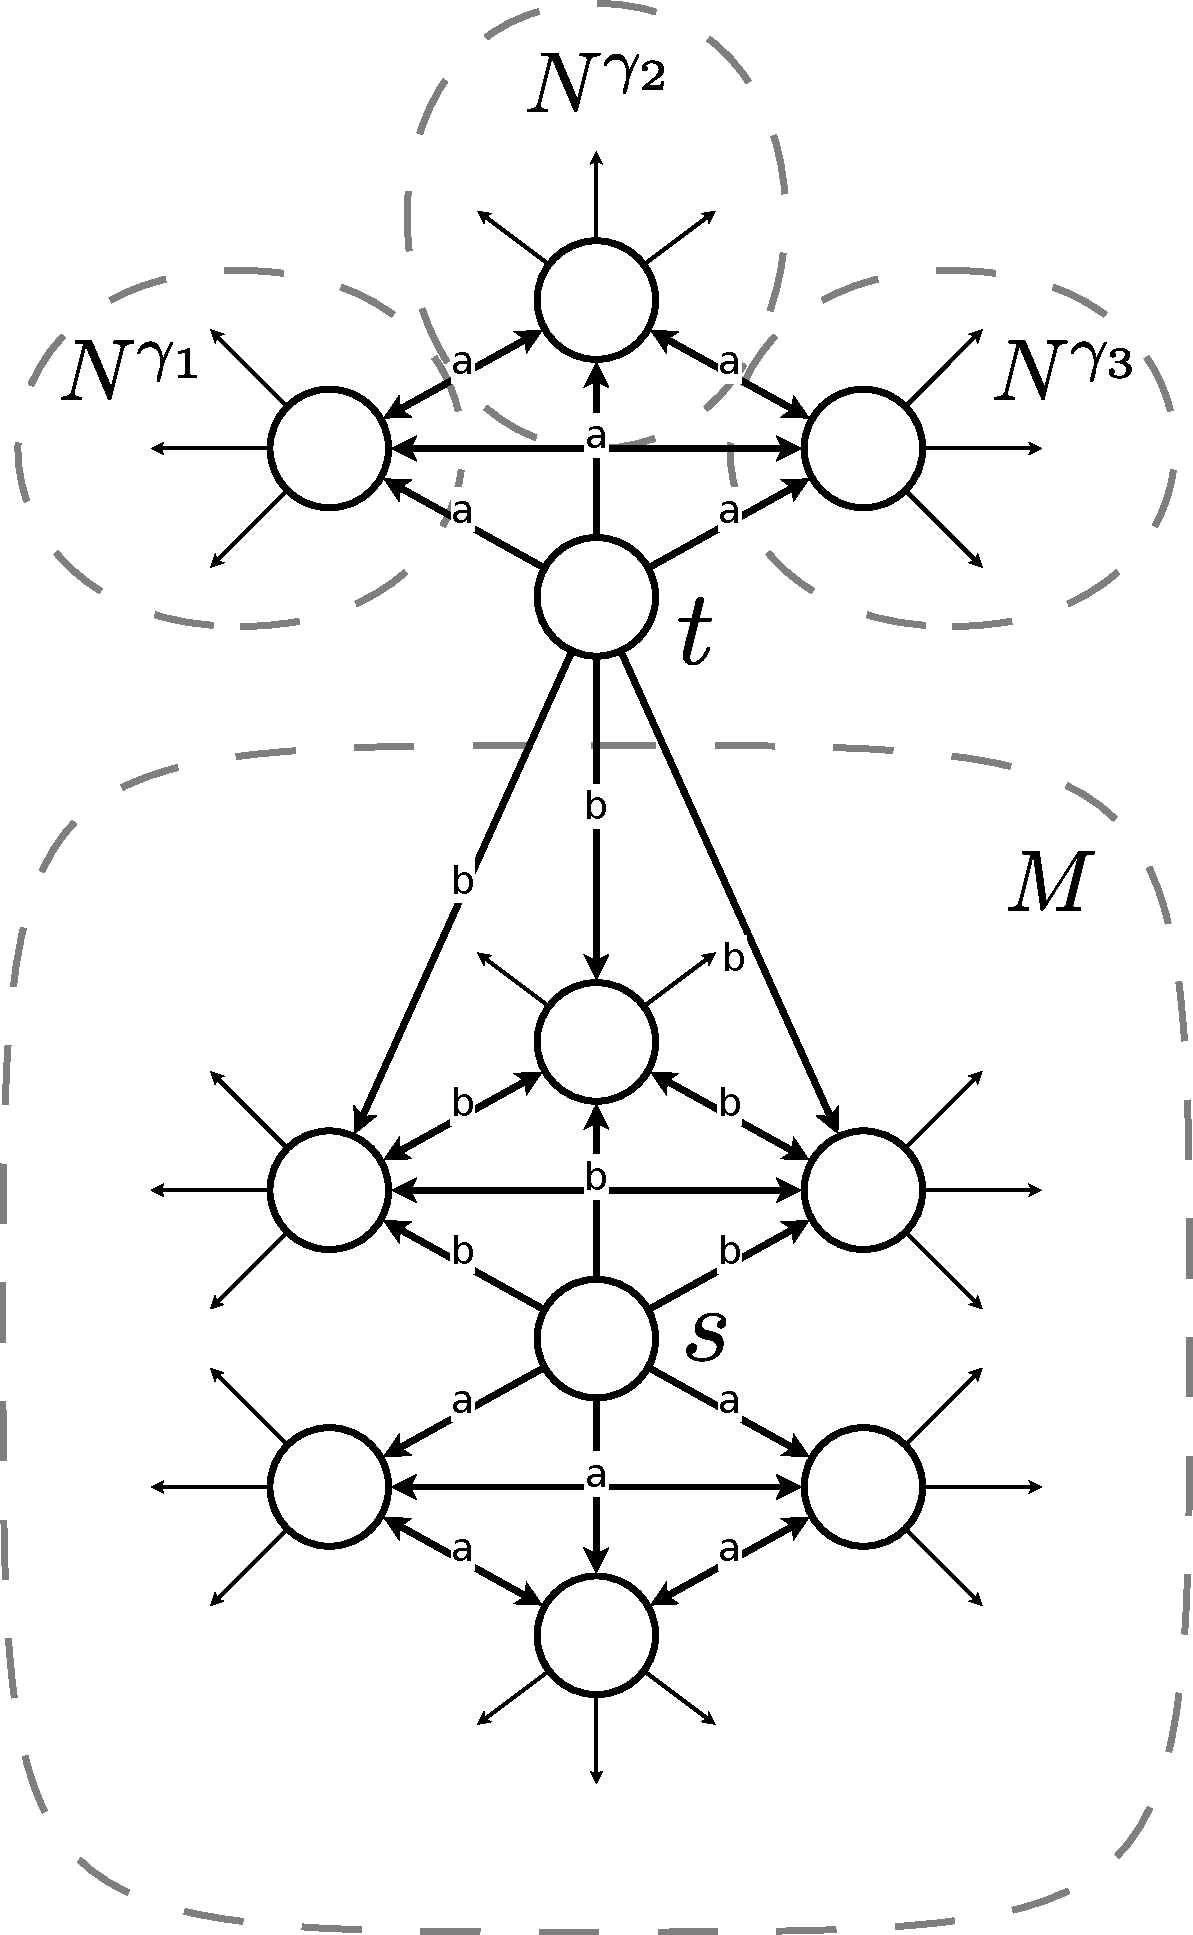
\includegraphics{rkd45}
}
\caption{
The model $N$ is constructed by taking the model $M$ and the models $N^\gamma$
for every $\gamma \in \Gamma$, and connecting them with an extra node $t$. $t$
is connected via an $a$-edge to $t^\gamma$ from each of the $N^\gamma$, and is
also connected via a $b$-edge to each $b$-successor of $s$ in $M$. We must also
have $a$-edges between each of the $t^\gamma$ to ensure that the resulting model
is transitive and Euclidean.
}
\end{center}
\end{figure}

We must show that $N$ is a doxastic model, that $N_t$ is an $a$-refinement of
$M_s$, and that for every $t^\gamma \in tR^N_a$ we have that $N_{t^\gamma}
\entails \gamma$. 

First we show that $N$ is a doxastic model. We must show two cases: that $R^N_a$
is serial, transitive and Euclidean, and that $R^N_b$ is also serial, transitive
and Euclidean, for every $b \in A - \{a\}$. As $M$ and each $N^\gamma$ are doxastic
models, the relations $R^M_c$ and $R^{N^\gamma}_c$ are serial, transitive and
Euclidean, for every $c \in A$. We observe that $S^N$ is a union of $\{t\}$,
$S^M$ and each $S^{N^\gamma}$. As $\Gamma$ is non-empty there is at
least one relationship $(t, t^\gamma)$ in $R^N_a$, therefore as $R^N_a$ also
contains $R^M_a$ and each $R^{N^\gamma}_a$, each of which are serial, then $R^N_a$
is also serial. Similarly, as $M$ is serial, $sR^M_b$ is non-empty, and so there
is at least one relationship $(t, t')$ where $t' \in sR^M_b$ in $R^N_b$;
therefore as $R^N_b$ also contains $R^M_b$ and $R^{N^\gamma}_b$, then $R^N_b$ is
also serial. To show the transitivity and Euclideaness of $R^N_a$, we first
observe that the relation can be considered in three independent parts; the
relationships between $t$ and $t^\gamma$, and between each $t^\gamma$; the
relation $R^M_a$; and the relations $R^{N^\gamma}_a$. The relation $R^M_a$ is
disjoint from the other relations, and so can be considered in isolation. By
hypothesis we have assumed that $t^\gamma R^{N^\gamma}_a = \{t^\gamma\}$, so as
there are no relationships from any $t^\gamma$ to a different state in
$S^{N^\gamma}$, we can also consider the each $R^{N^\gamma}_a$ separately from
the rest of $R^N_a$. We note that as $R^M_a$ and each $R^{N^\gamma}_a$ are
transitive and Euclidean, and as the remainder of the relation is essentially an
equivalence relation without the relationship $(t, t)$, it also has transitivity
and Euclideaness. Therefore $R^N_a$ is transitive and Euclidean. We can show
that $R^N_b$ is also transitive and Euclidean from the fact that $R^M_b$ and
each $R^{N^\gamma}_b$ is transitive and Euclidean, and otherwise disjoint from
each other, and the remainder of $R^N_b$ is simply a duplicate of relationships
from $s$ to its successors, then $R^N_b$ is also transitive and Euclidean.
Therefore $N$ is a doxastic model.

We next show that $N_t$ is an $a$-refinement of $M_s$. We construct an
$a$-simulation $\mathcal{R}$ from $N_t$ to $M_s$, where:

$$\mathcal{R} = \{(t, s)\} \cup \{(s', s') \mid s' \in S^M \} 
\cup \bigcup_{\gamma \in \Gamma} \mathcal{R}^\gamma$$

We must show that $\mathcal{R}$ satisfies {\bf atoms}, {\bf forth-$b$} for every
$b \in A$, and {\bf back-$b$} for every $b \in A - \{a\}$.

We note that, by construction, the valuation of $N$ matches the valuation of its
corresponding states in $M$ and each $N^\gamma$, and the valuation of $N_t$

We next show that $\mathcal{R}$ satisfies {\bf forth-$b$} for every $b \in A$.
Let $b \in A$, $u \in S^N$ and $v \in S^M$ such that $(u, v) \in \mathcal{R}$.
Suppose that $(u, v) \in \mathcal{R}^\gamma$ for some $\gamma \in \Gamma$.
Suppose further that $b = a$ and $u = t^\gamma$ for some $\gamma \in \Gamma$.
Then $t^\gamma R^N_a = tR^N_a = \{t^{\gamma'} \mid \gamma' \in \Gamma\}$.  As
$M$ is a doxastic model, we have that $s^\gamma R^M_a = sR^M_a = \{s^{\gamma'}
\mid \gamma' \in \Gamma\}$, and as each $\mathcal{R}^{\gamma'}$ is an
$a$-simulation between $N^{\gamma'}_{t^{\gamma'}}$ and $M_{s^{\gamma'}}$, we
have that for every $\gamma' \in \Gamma$, $(t^{\gamma'}, s^{\gamma'}) \in
\mathcal{R}^{\gamma'} \subseteq \mathcal{R}$. Otherwise consider any other $(u,
v) \in \mathcal{R}^\gamma$.  Then as $\mathcal{R}^\gamma$ is an $a$-simulation,
it satisfies {\bf forth-$b$} for every $b \in A$. Hence for every $u' \in
uR^{N^\gamma}_b$, there exists some $v' \in vR^M_b$ such that $(u', v') \in
\mathcal{R}^\gamma \subseteq \mathcal{R}$. Suppose that $b = a$ and $u =
t^\gamma$ for some $\gamma \in \Gamma$.  Suppose instead that $(u, v) = (s',
s')$ for some $s' \in S^M$.  Then we note that $s'R^N_b = s'R^M_b$, and hence
for every $s'' \in s'R^N_b$ we have that $s'' \in s'R^M_b$, and that $(s'', s'')
\in \mathcal{R}$. Finally suppose that $(u, u') = (t, s)$. Then suppose that $b
= a$. By construction, $tR^N_a = \{t^\gamma \mid \gamma \in \Gamma\}$, and hence
$v = t^\gamma$ for some $\gamma \in \Gamma$. Hence we can take $s^\gamma \in
sR^M_a$, and note that as $\mathcal{R}^\gamma$ is an $a$-simulation from
$M_{s^\gamma}$ to $N^\gamma_{t^\gamma}$, we know that $(t^\gamma, s^\gamma) \in
\mathcal{R}^\gamma \subseteq \mathcal{R}$. Suppose that $b \neq a$. Then by
construction, $tR^M_b = sR^M_b$, hence for every $t' \in tR^M_b$, we have that
$t' \in sR^M_b$, and hence we know that $(t', t') \in \mathcal{R}$. Hence
$\mathcal{R}$ satisfies {\bf back-$b$} for every $b \in A$.
matches that of $M_s$. Therefore $\mathcal{R}$ satisfies {\bf atoms}.

A similar argument to above shows that $\mathcal{R}$ satisfies {\bf forth-$b$}
for every $b \in A - \{a\}$.

Hence $\mathcal{R}$ is an $a$-simulation from $N_t$ to $M_s$. Thus $N_t
\refinement_a M_s$. 

We next show that for every $\gamma \in \Gamma$, we have that $N_{t^\gamma}
\entails \gamma$. As each $\gamma$ is an $a$-disjunctive normal formula, a
similar argument to that used in Lemma \ref{kd45-successors} can be used to
show that each of the successors of $N_{t^\gamma}$ are bisimilar to
corresponding successors of $N^\gamma_{t^\gamma}$ (trivially, as $N$ contains
no edges involving states in $S^{N^\gamma} - \{t^\gamma\}$, other than those in
$N^\gamma$), and therefore that $N_{t^\gamma} \entails \gamma$. 

As $N_t \refinement_a M_s$, and $N_t \entails \covers_a \Gamma$ we therefore
have that $M_s \entails \somerefs_a \covers_a \Gamma$.

Conversely, suppose that $M_s \entails \covers_a \Gamma$. Then there exists a
doxastic model $N_t \refinement_a M_s$, via some $a$-simulation $\mathcal{R}$,
such that $N_t \entails \covers_a \Gamma$. From the definition of the cover
operator, this implies that $N_t \entails \knows_a \bigvee_{\gamma \in \Gamma}
\gamma \land \bigwedge_{\gamma \in \Gamma} \suspects_a \gamma$. In particular we
note that for every $\gamma \in \Gamma$, $N_t \entails \suspects_a \gamma$, and
so there exists some $t^\gamma \in tR^N_a$ such that $N_{t^\gamma} \entails
\gamma$. As $t^\gamma \in tR^N_a$, and $(t, s) \in \mathcal{R}$, by {\bf
forth-$a$} there exists some $s^\gamma \in sR^M_a$ such that $(t^\gamma, s^\gamma)
\in \mathcal{R}$. Hence $\mathcal{R}$ is also an $a$-simulation from
$N_{t^\gamma}$ to $M_{s^\gamma}$, and so $M_{s^\gamma} \entails \somerefs_a
\gamma$. As for every $\gamma \in \Gamma$ we have that $s^\gamma \in sR^M_a$, we
also have that $M_s \entails \suspects_a \somerefs_a \gamma$. Therefore we
finally have that $M_s \entails \bigwedge_{\gamma \in \Gamma} \suspects_a
\somerefs_a \gamma$.

Therefore {\bf RKD45} is sound.

\paragraph{RComm} 
Suppose that $M_s$ is a doxastic model such that $M_s \entails \covers_b \{
\somerefs_a \gamma \mid \gamma \in \Gamma\}$, where $a \ne b$ and $\Gamma$ is a
set of $b$-disjunctive normal formulae. From the definition of the cover
operator, this implies that $M_s \entails \knows_b \bigvee_{\gamma \in \Gamma}
\somerefs_a \gamma \land \bigwedge_{\gamma \in \Gamma} \suspects_b \somerefs_a
\gamma$. In particular, we note that for every $\gamma \in \Gamma$, there
exists some $s^\gamma \in sR^M_b$ such that $M_{s^\gamma} \entails \somerefs_a
\gamma$.  Then there exists a doxastic model $N^\gamma_{t^\gamma} \refinement_a
M_{s^\gamma}$, via some $a$-simulation $\mathcal{R}^\gamma$, such that
$N^\gamma_{t^\gamma} \entails \gamma$. Without loss of generality, as $\gamma$
is a $b$-disjunctive normal formula, we may assume that $t^\gamma
R^{N^\gamma}_b = \{t^\gamma\}$ (by Lemma \ref{kd45-successors}), and that the
$N^\gamma$ are disjoint.

Let $t$ be a state such that $t \notin S^{N^\gamma}$ for every $\gamma \in
\Gamma$. Then we construct a Kripke model $N = (S^N, R^N, V^N)$, where:

\begin{eqnarray*}
S^N &=& \{t\} \cup S^M \bigcup_{\gamma \in \Gamma} S^{N^\gamma}\\
R^N_b &=& \{(t, t^\gamma) \mid \gamma \in \Gamma\} \cup \{(t^\gamma,
t^{\gamma'}) \mid \gamma, \gamma' \in \Gamma\} \cup R^M_b \cup \bigcup_{\gamma
\in \Gamma} R^{N^\gamma}_b\\
R^N_c &=& \{(t, t') \mid t' \in sR^M_c\} \cup R^M_c \cup \bigcup_{\gamma \in
\Gamma} R^{N^\gamma}_c \text{ for $c \in A - \{b\}$}\\
V^N(p) &=& 
\begin{cases}
\{t\} \cup V^M(p) \cup \bigcup_{\gamma \in \Gamma} V^{N^\gamma}(p) & \text{if $s
\in V^M(p)$}\\
V^M(p) \cup \bigcup_{\gamma \in \Gamma} V^{N^\gamma}(p) & \text{otherwise}
\end{cases}
\text{ for $p \in P$}
\end{eqnarray*}

We note that $N$ is a doxastic model, by similar arguments as used in the proof
for {\bf RKD45}.

We next construct an $a$-simulation $\mathcal{R}$ from $N_t$ to $M_s$, where:

$$\mathcal{R} = \{(t, s)\} \cup \{(s', s') \mid s' \in S^M\} \cup \bigcup_{\gamma \in \Gamma} \mathcal{R}^\gamma$$

We note that $\mathcal{R}$ is an $a$-simulation, by similar arguments as used in
the proof for {\bf RKD45}. In particular, this means that $N_t \refinement_a
M_s$.

We also note that for every $\gamma \in \Gamma$ that $N_{t^\gamma} \bisim
N^\gamma_{t^\gamma}$, by similar arguments as used in the proof for {\bf RKD45}.
In particular, this means that as $N^\gamma_{t^\gamma} \entails \gamma$ that we
also have $N_{t^\gamma} \entails \gamma$, for every $\gamma \in \Gamma$.
Therefore $N_t \entails \covers_b \Gamma$.

Therefore $M_s \entails \somerefs_a \covers_b \Gamma$.

The converse, $\somerefs_a \covers_b \Gamma \implies \covers_b \{\somerefs_a
\gamma \mid \gamma \in \Gamma\}$ follows a similar proof to the relevant part in
the proof for {\bf RKD45}.

Therefore {\bf RComm} is sound.

\paragraph{RDist} 
Suppose that $M_s$ is a doxastic model such that $M_s
\entails \bigwedge_{b \in A} \somerefs_a \covers_b \Gamma_b$, where $\Gamma_b$
is a set of $b$-disjunctive formulae for each $b \in A$.

Then as $a \in A$, we have that $M_s \entails \somerefs_a \covers_a \Gamma_a$,
and by {\bf RKD45} this implies that $M_s \entails \bigwedge_{\gamma \in
\Gamma_a} \suspects_a \somerefs_a \gamma$. We also have for every $b \in A -
\{a\}$ that $M_s \entails \somerefs_a \covers_b \Gamma_b$, and by {\bf RComm}
this implies that $M_s \entails \covers_b \{\somerefs_a \gamma \mid \gamma \in
\Gamma_b\}$, and by the definition of the cover operator implies that $M_s
\entails \bigwedge_{\gamma \in \Gamma_b} \suspects_b \somerefs_a \gamma$.  Hence
for every $b \in A$ and $\gamma \in \Gamma_b$, we have that $\suspects_b
\somerefs_a \gamma$. This implies that for each $b \in A$ and each $\gamma \in
\Gamma_b$ that there exists some $t^{\gamma} \in sR^M_b$ such that $M_{t^\gamma}
\entails \somerefs_a \gamma$. Therefore there exists a doxastic model
$N^\gamma_{t^\gamma} \refinement_a M_{t^\gamma}$, via some $a$-simulation
relation $\mathcal{R}^\gamma$, such that $N^\gamma_{t^\gamma} \entails \gamma$.
Without loss of generality, as $\gamma$ is a $b$-disjunctive normal formula, we
may assume that $t^\gamma R^{N^\gamma}_b = \{t^\gamma\}$ (by Lemma
\ref{kd45-successors}), and that the $N^\gamma$ are disjoint.

Let $t \notin S^{N^\gamma}$ for every $\gamma \in \Gamma$.
Then we construct a Kripke model $N = (S, R^N, V^N)$ where:

\begin{eqnarray*}
S^N &=& \{t\} \cup \bigcup_{b \in A, \gamma \in \Gamma_b} S^{N^\gamma}\\
R^N_b &=& \{(t, t^{\gamma}) \mid b \in A, \gamma \in \Gamma_b\} 
\cup \{(t^\gamma, t^{\gamma'}) \mid \gamma, \gamma' \in \Gamma_b\}
\cup \bigcup_{b \in A, \gamma \in \Gamma_b} R^{N^\gamma}_b \text{ for $b \in A$}\\
V^N(p) &=& 
\begin{cases}
\{t\} \cup \bigcup_{b \in A, \gamma \in \Gamma_b} V^{N^\gamma}(p) & \text{if $s
\in V^M(p)$}\\
\bigcup_{b \in A, \gamma \in \Gamma_b} V^{N^\gamma}(p) & \text{otherwise}
\end{cases}
\end{eqnarray*}

We note that $N$ is a doxastic model, by similar arguments as used in the proof
for {\bf RKD45}.

We next construct an $a$-simulation $\mathcal{R}$ from $N_t$ to $M_s$, where:

$$\mathcal{R} = \{(t, s)\} \cup \bigcup_{b \in A, \gamma \in \Gamma_b}
\mathcal{R}^\gamma$$

We note that this is an $a$-simulation, by similar arguments as used in the
proof for {\bf RKD45}. In particular, this means that $N_t \refinement_a M_s$.

We also note that for every $b \in A$, and $\gamma \in \Gamma_b$ that
$N_{t^\gamma} \bisim N^\gamma_{t^\gamma}$, by similar arguments as used in the
proof for {\bf RKD45}. In particular, this means that as $N^\gamma_{t^\gamma}
\entails \gamma$ that we also have $N_{t^\gamma} \entails \gamma$, for every $b
\in A$ and $\gamma \in \Gamma_b$. Therefore $N_t \entails \covers_b \Gamma_b$
for every $b \in A$, and therefore $N_t \entails \bigwedge_{b \in A} \covers_b
\Gamma_b$.

Therefore $M_s \entails \somerefs_a \bigwedge_{b \in A} \covers_b \Gamma_b$ and
{\bf RDist} is sound.

Therefore the axiomatisation \axiomKDF{} is sound.
\end{proof}

\begin{lemma}
The following is derivable in \axiomKDF{}.

$$
\proves \bigwedge_{b \in A} \somerefs_a \covers_b \Gamma_b \iff
\somerefs_a \bigwedge_{b \in A} \covers_b \Gamma_b \\
$$
where $\Gamma_b$ is a set of $b$-disjunctive normal formulae for
every $b \in A$.
\end{lemma}

\begin{proof}
The forward direction is the axiom {\bf RDist}. 

The converse can be derived in a more general form as $\somerefs_a (\phi \land
\psi) \implies \somerefs_a \phi \land \somerefs_a \psi$. The derivation is
similar to the derivation for $\knows_a (\phi \land \psi) \implies \knows_a \phi
\land \knows_a \psi$ in the modal logic \logicK{}, using the axiom {\bf R} in
place of {\bf K}.
\end{proof}

\begin{lemma}\label{kd45-translation}
Every formula of \logicKDF{} is provably equivalent to a formula of \logicKD{}.
\end{lemma}

\begin{proof}
Given a formula $\psi$ we prove by induction on the number of occurrences of
\somerefs{} that $\psi$ is equivalent to a \somerefs-free formula, and
therefore to a formula in \logicKD{}. The base case with no \somerefs operators
is trivial, as a \somerefs-free formula is a formula in \logicKD{}. Now assume
that $\psi$ contains $n + 1$ \somerefs-operators. Choose a subformula of type
$\somerefs_a \phi$ of our given formula, where $\phi$ is \somerefs-free. Without
loss of generality, by Lemma~\ref{kd45-cdnf} we can assume that $\phi$ is in
cover logic disjunctive normal form.  We prove by induction on the structure of
$\phi$ that $\somerefs_a \phi$ is provably equivalent to a formula $\chi$ without
the $\somerefs_a$ operator.

\begin{itemize}
\item $\somerefs_a (\phi \lor \psi)$ iff $\somerefs \phi \lor \somerefs \psi$.
(Derivable from {\bf P} and {\bf R})
\item $\somerefs_a (\pi \land \bigwedge_{b \in A} \covers_b \Gamma_b)$ iff
$\pi \land \bigwedge_{\gamma \in \Gamma_a} \suspects_a \somerefs_a \gamma \land
\bigwedge_{b \in A - \{a\}} \covers_b \{\somerefs_a \gamma \mid \gamma \in
\Gamma_b\}$ (Derivable from {\bf P}, {\bf R}, {\bf RP}, {\bf RDist}, {\bf
RKD45} and {\bf RComm})
\end{itemize}

Replacing $\somerefs_a \phi$ with $\chi$ in $\psi$ gives an equivalent formula
with one less \somerefs-operator. Thus by induction, all formulae in
\logicKDF{} can be translated into an equivalent formula in
\logicKD{}.
\end{proof}

The rest of the completeness proof is merely a formality to show that, given the
above translation into \logicKD{}, we can show completeness by using these
translations along with the completeness of \logicKD{}.

\begin{corollary}\label{kd45-derivable}
Let $\phi \in \logicKDF$ be given and $\psi \in \logicKD$ be semantically
equivalent to $\phi$.  If $\psi$ is a theorem in \logicKD{}, then $\phi$ is a
theorem in \axiomKDF{}.
\end{corollary}

\begin{proof}
Let $\phi \in \logicKDF$ and let $\psi \in \logicKD$ be semantically equivalent to
$\phi$. By Lemma~\ref{kd45-translation}, we can obtain some $\phi' \in \logicKD$
that is semantically equivalent to $\phi$ (and thus also to $\psi$) by following
the given translation steps. We can extend a derivation of $\psi$ to a
derivation of $\phi'$ as the two are semantically equivalent in \logicKD{}, and by
the completeness of \logicKD{} this equivalence is derivable. As \axiomKDF{} is a
conservative extension of \logicKD{}, this equivalence is therefore also derivable
in \axiomKDF{}. The derivation can be further extended to $\phi$ by observing that all
of the reduction steps in Lemma~\ref{kd45-translation} are provable equivalences
in \axiomKDF{}. Therefore $\phi$ is a theorem in \axiomKDF{}.
\end{proof}

\begin{lemma}\label{kd45-complete}
The axiom schema \axiomKDF{} is complete for the logic \logicKDF{}.
\end{lemma}

Note that as we are discussing derivability in two different logics in the
following proof, we use a subscript on the turnstile symbol to denote the logic
we are working in (e.g. $\proves_{\logicKDF}$)

\begin{proof}
Let $\phi \in \logicKDF$ such that $\entails_{\logicKDF} \phi$. Then by
Lemma~\ref{kd45-translation}, there exists a semantically equivalent formula
$\psi \in \logicKD$ which is \somerefs-free. As $\entails_{\logicKDF} \phi$ and
$\phi \iff \psi$, then $\entails_{\logicKDF} \psi$. As $\psi$ is
\somerefs-free, then it follows that $\entails_{\logicKD} \psi$, and by the
completeness of \axiomKDF{} it follows that $\proves_{\logicKD} \psi$.
Therefore by Corollary~\ref{kd45-derivable} we have that $\proves_{\logicKDF}
\phi$.
\end{proof}

\begin{theorem}
The axiomatisation \axiomKDF{} is sound and complete for the logic \logicKDF{}.
\end{theorem}

\begin{proof}
The soundness proof is given in Lemma~\ref{kd45-sound} and the completeness
proof is given in Lemma~\ref{kd45-complete}.
\end{proof}

\chapter{Epistemic logic}\label{chapter-epistemic}

\section{Syntax and semantics}

Here we define the syntax and semantics of the logic \logicSF{}, which
restricts the logic \logicKF{}, as defined by van Ditmarsch and
French~\cite{french2009simulation}, to deal with only models and refinements of
epistemic models.

% TODO - more motiviation

\begin{definition}[Language of \langF{}] % TODO - move to the K section
Given a finite set of agents $A$ and a set of propositional atoms $P$, the
language of \langF{} is defined by the following abstract syntax:

$$
\phi ::=    p \bnfalt
            \neg \phi \bnfalt
            \phi \land \phi \bnfalt
            \knows_a \phi \bnfalt
            \allrefs_a \phi
$$
where $a \in A$ and $p \in P$.
\end{definition}

Standard abbreviations include:
$\top ::= \phi \lor \neg \phi$;
$\bot ::= \neg \top$;
$\phi \lor \psi ::= \neg (\neg \phi \land \neg \psi)$;
$\phi \implies \psi ::= \neg \phi \lor \psi$;
and $\suspects_a \phi ::= \neg \knows_a \neg \phi$.
We use an abbreviation for the dual of the $\allrefs_a$ operator,
$\somerefs_a \phi ::= \neg \allrefs_a \neg \phi$.

We also use the cover operator $\covers_a \Gamma$, where $\Gamma$ is a finite
set of formulae, which is an abbreviation for 
$\covers_a \Gamma ::= \knows_a \bigvee_{\gamma \in \Gamma} \gamma \land
\bigwedge_{\gamma \in \Gamma} \suspects_a \gamma$. The cover operator is relied
on for our axiomatisation, in much the same way it is relied on for the
axiomatisation of \logicKiF{} presented by van Ditmarsch, French and
Pinchinat~\cite{french2010future}. % TODO - include citation for cover operator

\begin{definition}[Semantics of \logicSF{}]
Let $M = (S, R, V)$ be a doxastic model. The interpretation of $\phi \in
\logicKDF$ is defined inductively.

\begin{eqnarray*}
M_s &\entails& p \text{ iff } s \in V_p\\
M_s &\entails& \neg \phi \text{ iff } M_s \nentails \phi\\
M_s &\entails& \phi \land \psi \text{ iff } M_s \entails \phi \text{ and } M_s
\entails \psi\\
M_s &\entails& \knows_a \phi \text{ if for all } t \in S : (s, t) \in R_a \text{
implies } M_t \entails \phi\\
M_s &\entails& \allrefs_a \phi \text{ iff for all } M'_{s'} \in \classS : M_s
\simulation_a M'_{s'} \text{ implies } M'_{s'} \entails \phi\\
\end{eqnarray*}
\end{definition}

The differences between \logicKF{} and \logicSF{} are similar to the differences
between \logicKF{} and \logicKDF{} discussed earlier. The class of models that
these logics are interpreted over are different, and particularly the
interpretation of the refinement operator means that \logicSF{} is not a
conservative extension of \logicKF{}. The example given earlier for \logicKDF{}
applies also to \logicSF{}: whilst $\somerefs_a \knows_a \bot$ is valid in
\logicKF{}, due to the reflexive nature of models in \classS{}, it is not valid
in \logicSF{}.

\begin{lemma}
The logic \logicSF{} is bisimulation invariant.
\end{lemma}

The proof for the bisimulation invariance of \logicKF{}, given by van Ditmarsch,
French and Pinchinat~\cite{french2010future} also applies to \logicKDF{}. 
% TODO - more explanation?

% TODO - examples

\section{Decision procedures}


\bibliographystyle{plain}
\bibliography{thesis}

\end{document}
